% !TEX encoding = UTF-8 Unicode
% \documentclass[mathserif]{beamer}
% %\usepackage{CJKutf8}
% %\usepackage{xeCJK}
% %\usepackage{xeCJK}
% %\setCJKmainfont[BoldFont=STZhongsong, ItalicFont=STKaiti]{STSong}
% %\setCJKsansfont[BoldFont=STHeiti]{STXihei}
% %\setCJKmonofont{STsong}

% %\usetheme{default}
% %\usetheme{AnnArbor}
% %\usetheme{Antibes}
% %\usetheme{Bergen}
% %\usetheme{Berkeley}
% %\usetheme{Berlin}
% \usetheme{Boadilla}
% %\usetheme{CambridgeUS}
% %\usetheme{Copenhagen}
% %\usetheme{Darmstadt}
% %\usetheme{Dresden}
% %\usetheme{Frankfurt}
% %\usetheme{Goettingen}
% %\usetheme{Hannover}
% %\usetheme{Ilmenau}
% %\usetheme{JuanLesPins}
% %\usetheme{Luebeck}
% %\usetheme{Madrid}
% %\usetheme{Malmoe}
% %\usetheme{Marburg}
% %\usetheme{Montpellier}
% %\usetheme{PaloAlto}
% %\usetheme{Pittsburgh}
% %\usetheme{Rochester}
% %\usetheme{Singapore}
% %\usetheme{Szeged}
% %\usetheme{Warsaw}

% % As well as themes, the Beamer class has a number of color themes
% % for any slide theme. Uncomment each of these in turn to see how it
% % changes the colors of your current slide theme.

% %\usecolortheme{albatross}
% %\usecolortheme{beaver}
% %\usecolortheme{beetle}
% %\usecolortheme{crane}
% %\usecolortheme{dolphin}
% %\usecolortheme{dove}
% %\usecolortheme{fly}
% %\usecolortheme{lily}
% %\usecolortheme{orchid}
% %\usecolortheme{rose}
% %\usecolortheme{seagull}
% %\usecolortheme{seahorse}
% \usecolortheme{sidebartab}
% %\usecolortheme{whale}
% %\usecolortheme{wolverine}
% \textsl{•}
\documentclass[10pt, mathserif]{beamer} %, mathserif
\renewcommand{\baselinestretch}{1.3}
\usepackage{bbm,tikz}
\usetheme{boxes}
\usecolortheme{rose}
\usepackage{multirow}
%\usetheme{Berlin}
%\usefonttheme{serif}
\setbeamertemplate{blocks}[rounded][shadow=false]
\setbeamertemplate{footline}[frame number]
\newtheorem{assumption}{Assumption}
\newtheorem{thm}{Theorem}
\newtheorem{prop}{Proposition}
\newtheorem{col}{Corollary}
\newtheorem{lem}{Lemma}
\newtheorem*{obs}{Observation}
\theoremstyle{definition}
\newtheorem{defn}{Definition}
\newtheorem{axiom}{Axiom}
\newtheorem{hyp}{Hypothesis}
\theoremstyle{plain}
\setbeamertemplate{theorems}[numbered]
\usetikzlibrary{decorations.pathreplacing}
\newenvironment{sequation}{\small\begin{equation}}{\end{equation}}
\newenvironment{sequation*}{\small\begin{equation*}}{\end{equation*}}
\newenvironment{tequation}{\tiny\begin{equation}}{\end{equation}}
\newenvironment{tequation*}{\tiny\begin{equation*}}{\end{equation*}}
\usepackage{pstricks,egameps}
\newcommand*{\KeepStyleUnderBrace}[1]{%f
\mathop{%
\mathchoice
{\underbrace{\displaystyle#1}}%
{\underbrace{\textstyle#1}}%
{\underbrace{\scriptstyle#1}}%
{\underbrace{\scriptscriptstyle#1}}%
}\limits
}
\usepackage{pifont}
\newcommand{\cmark}{\ding{51}}%
\newcommand{\xmark}{\ding{55}}%
\usepackage{pgfpages}
\usepackage[ruled]{algorithm2e}
%\setbeameroption{show notes on second screen}
\setbeameroption{hide notes}
\setbeamertemplate{note page}{%
  \insertnote%
}
\usepackage{lmodern}
\setlength{\leftmargini}{0pt}
\setlength{\leftmarginii}{14pt}

\usepackage{dsfont}
\usepackage{wrapfig}
\usepackage{mathrsfs}

\def\caliP{\mathscr{P}_{\textup{sgn}}}


\usepackage{mathtools}
\mathtoolsset{showonlyrefs}
\usepackage{appendixnumberbeamer}
\usepackage{appendix}

\usepackage{natbib}
\usepackage{graphicx}
\usepackage{setspace}

\usepackage{empheq}


    \title{Nonparametric Tensor Completion via Sign Series}
    %\subtitle{Who did U.S. Workers lose job to?}
    \author{Chanwoo Lee\\ Joint work with Miaoyan Wang}

    \institute{\scriptsize Department of Statistics \\University of Wisconsin - Madison}
    \date{\small{992 Seminar, Feb 3, 2021}}
\AtBeginSection[]

\usepackage{bm}
\input macros.tex

\begin{document}
%\begin{CJK*}{UTF8}{gbsn}
\renewcommand{\raggedright}{\leftskip=0pt \rightskip=0pt plus 0cm}

\begin{frame}[plain]{}{}
\titlepage
\end{frame}



\section{Introduction}
\begin{frame}[label = slide1]
    \frametitle{Introduction: what is a tensor?}
    \begin{itemize}
        \item Tensors are generalizations of vectors and matrices:
        \begin{center}
            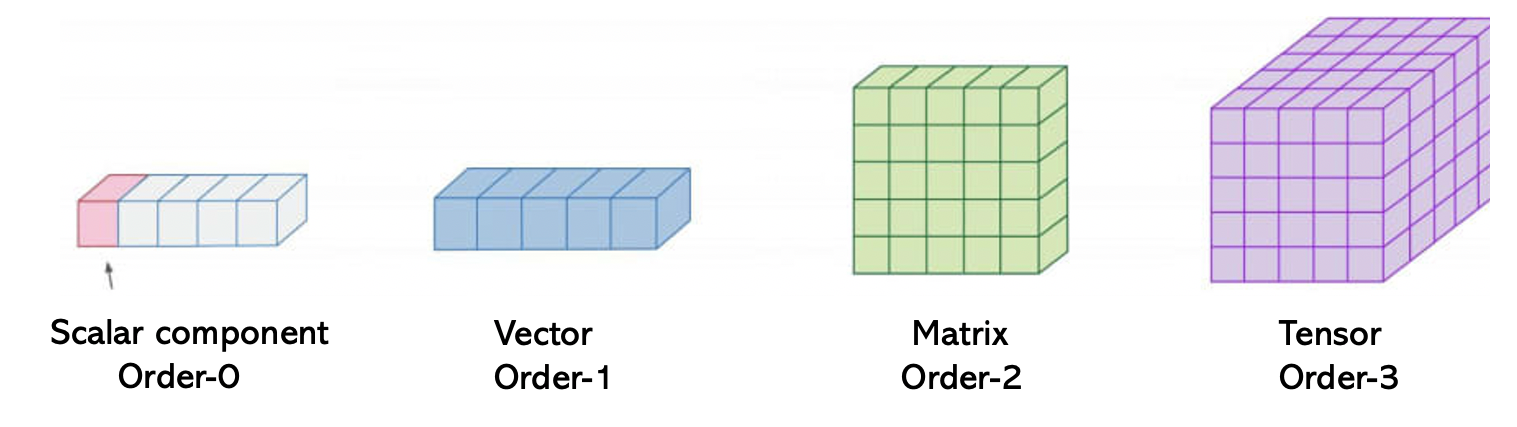
\includegraphics[width=9cm]{tensorimage.png}
        \end{center}
         \item We focus on tensors of order 3 or greater, also called {\color{red}{higher-order tensors.} }
        \item Denote an order-$K (d_1,\cdots,d_K)$ dimensional tensor as $\mathcal{Y} = \entry{y_\omega}\in\mathbb{R}^{d_1\times\cdots\times d_K}$ \\
        where $\omega \in [d_1]\times \cdots\times [d_K].$
    \end{itemize}
\end{frame}





\begin{frame}{Introduction: Tucker decomposition}
\begin{itemize}
    \item Tucker decomposition~\citep{de2000multilinear}.
    \begin{itemize}
    \item $\mathcal{Y} = \mathcal{C}\times_1 \mM_1\times_2 \mM_2 \times_3 \mM_3$.
    \item Generalization of matrix SVD to higher orders: $\mY = \mU\Sigma\mV^T (=\Sigma\times_1\mU\times_2\mV)$
    \item Tucker rank of an order-3 tensor is defined as
    \vspace{-0.3cm}
    \begin{align*}
    r(\mathcal{Y}) &= (r_1,r_2,r_3).
    \end{align*}
   
    \begin{center}
    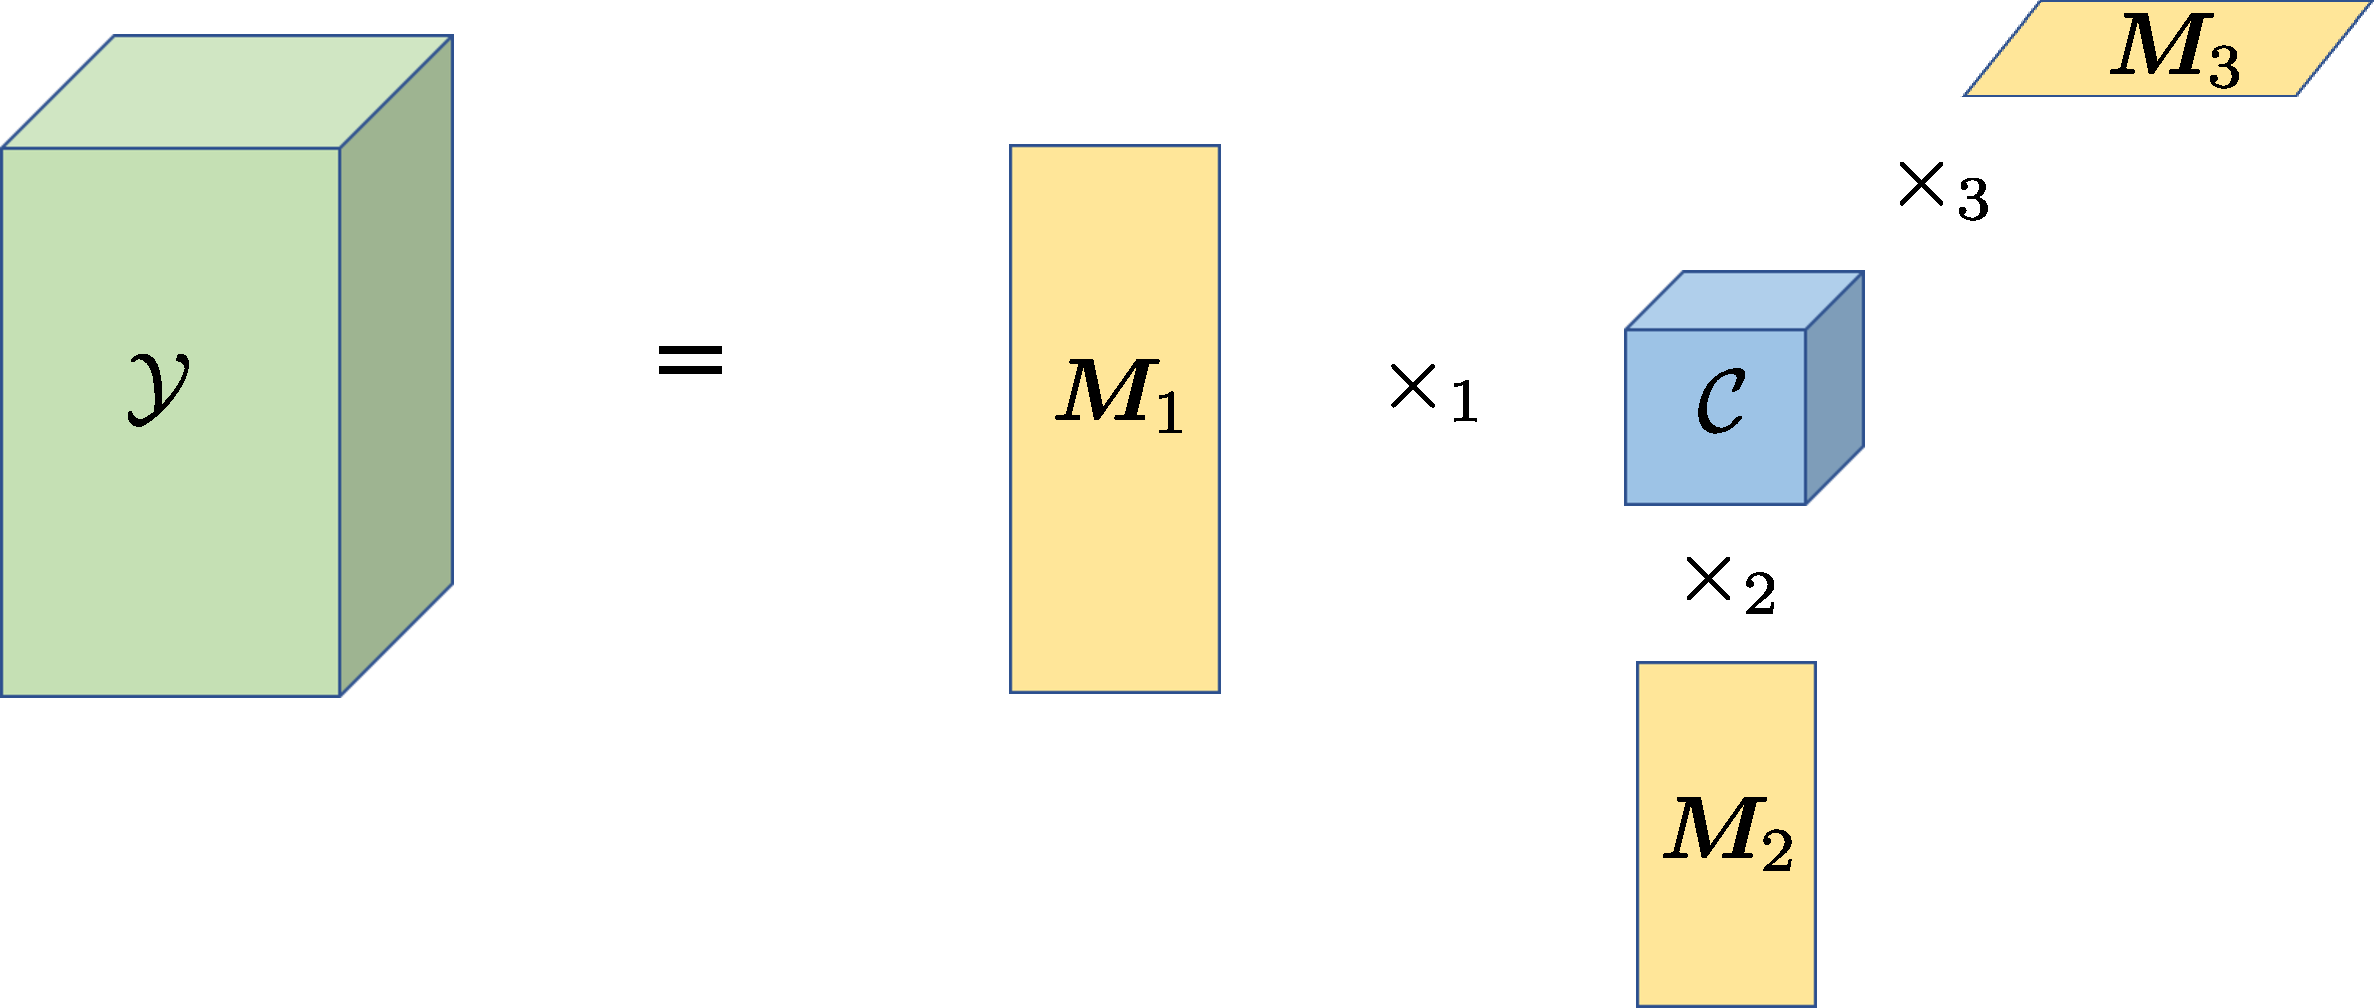
\includegraphics[width = 10cm]{tucker.pdf}
    \end{center}
    \end{itemize}
\end{itemize}
\end{frame}


\begin{frame}{Introduction:  Canonical Polyadic (CP) decomposition}
\begin{itemize}
    \item CP decomposition~\citep{hitchcock1927expression}.
    \begin{itemize}
    \item $\mathcal{Y} = \sum_{s = 1}^r\lambda_s\ma_s^{(1)}\otimes \cdots\otimes \ma_s^{(K)}$.
    
    \item Generalization of matrix SVD to higher orders: $\mY = \sum_{s = 1}^r \lambda_s \bm u_s\otimes \mv_s$
    \item CP rank is defined as the minimal $r$ for which the above equation holds.
    \item Today, we use the tensor rank as CP rank.
    \begin{center}
    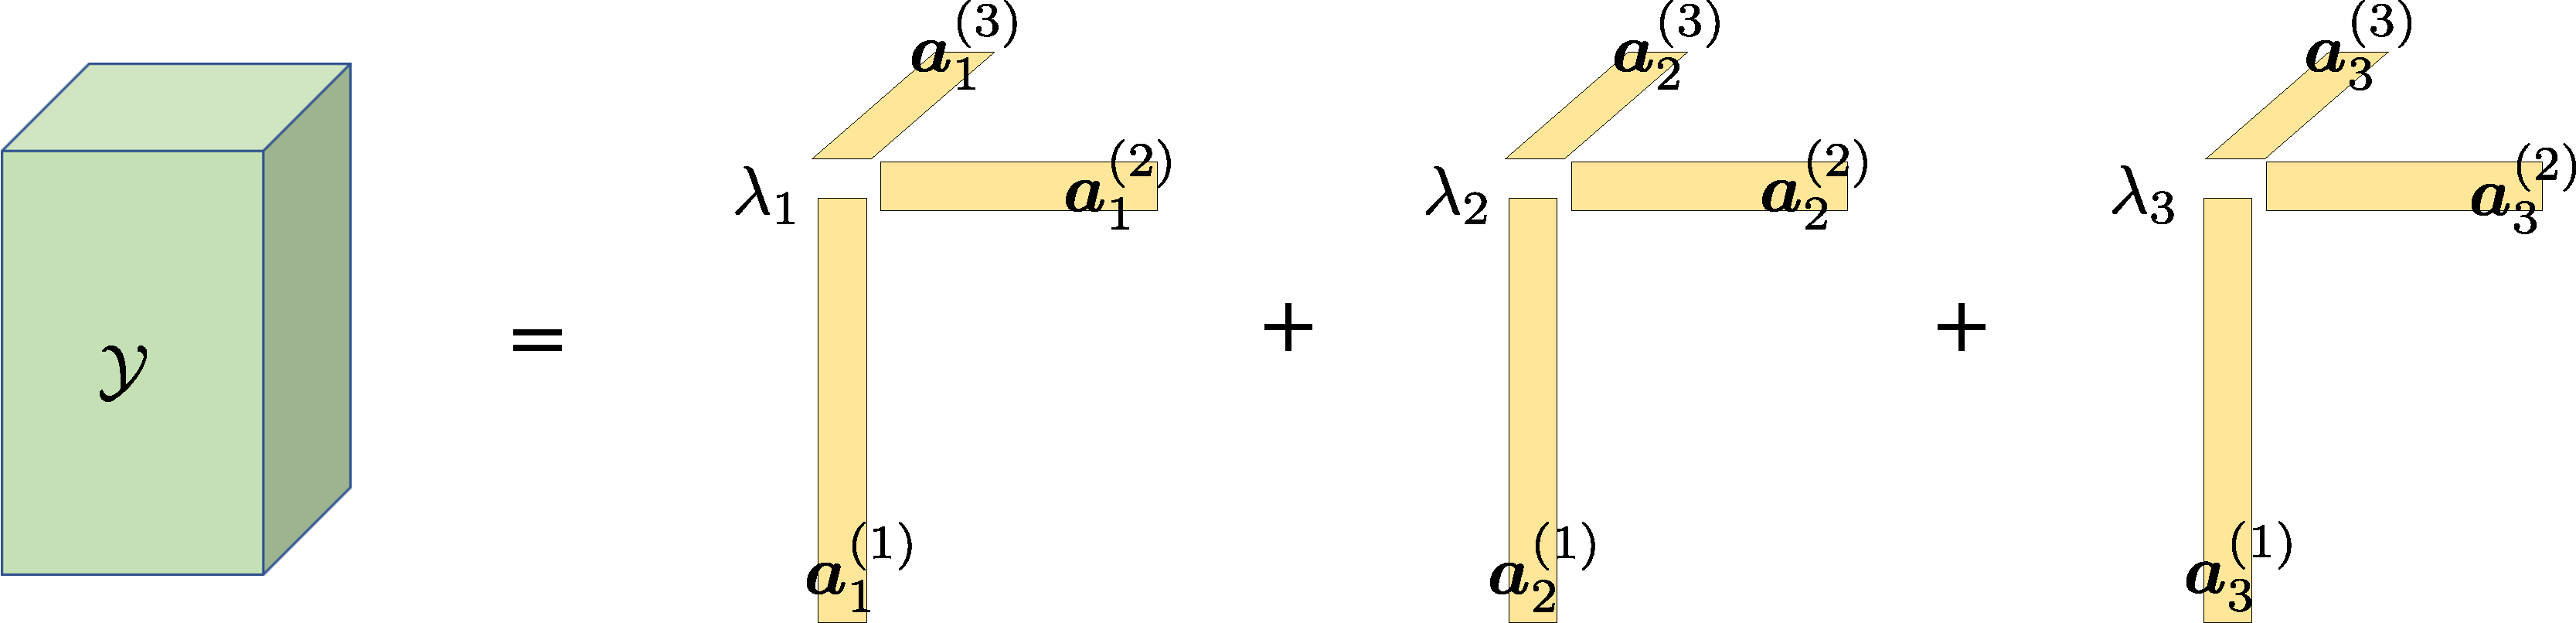
\includegraphics[width = \textwidth]{cpdecomp.pdf}
    \end{center}
    \end{itemize}
\end{itemize}
\end{frame}

\begin{frame}{Main problems: the signal plus noise model}
     \begin{center}
    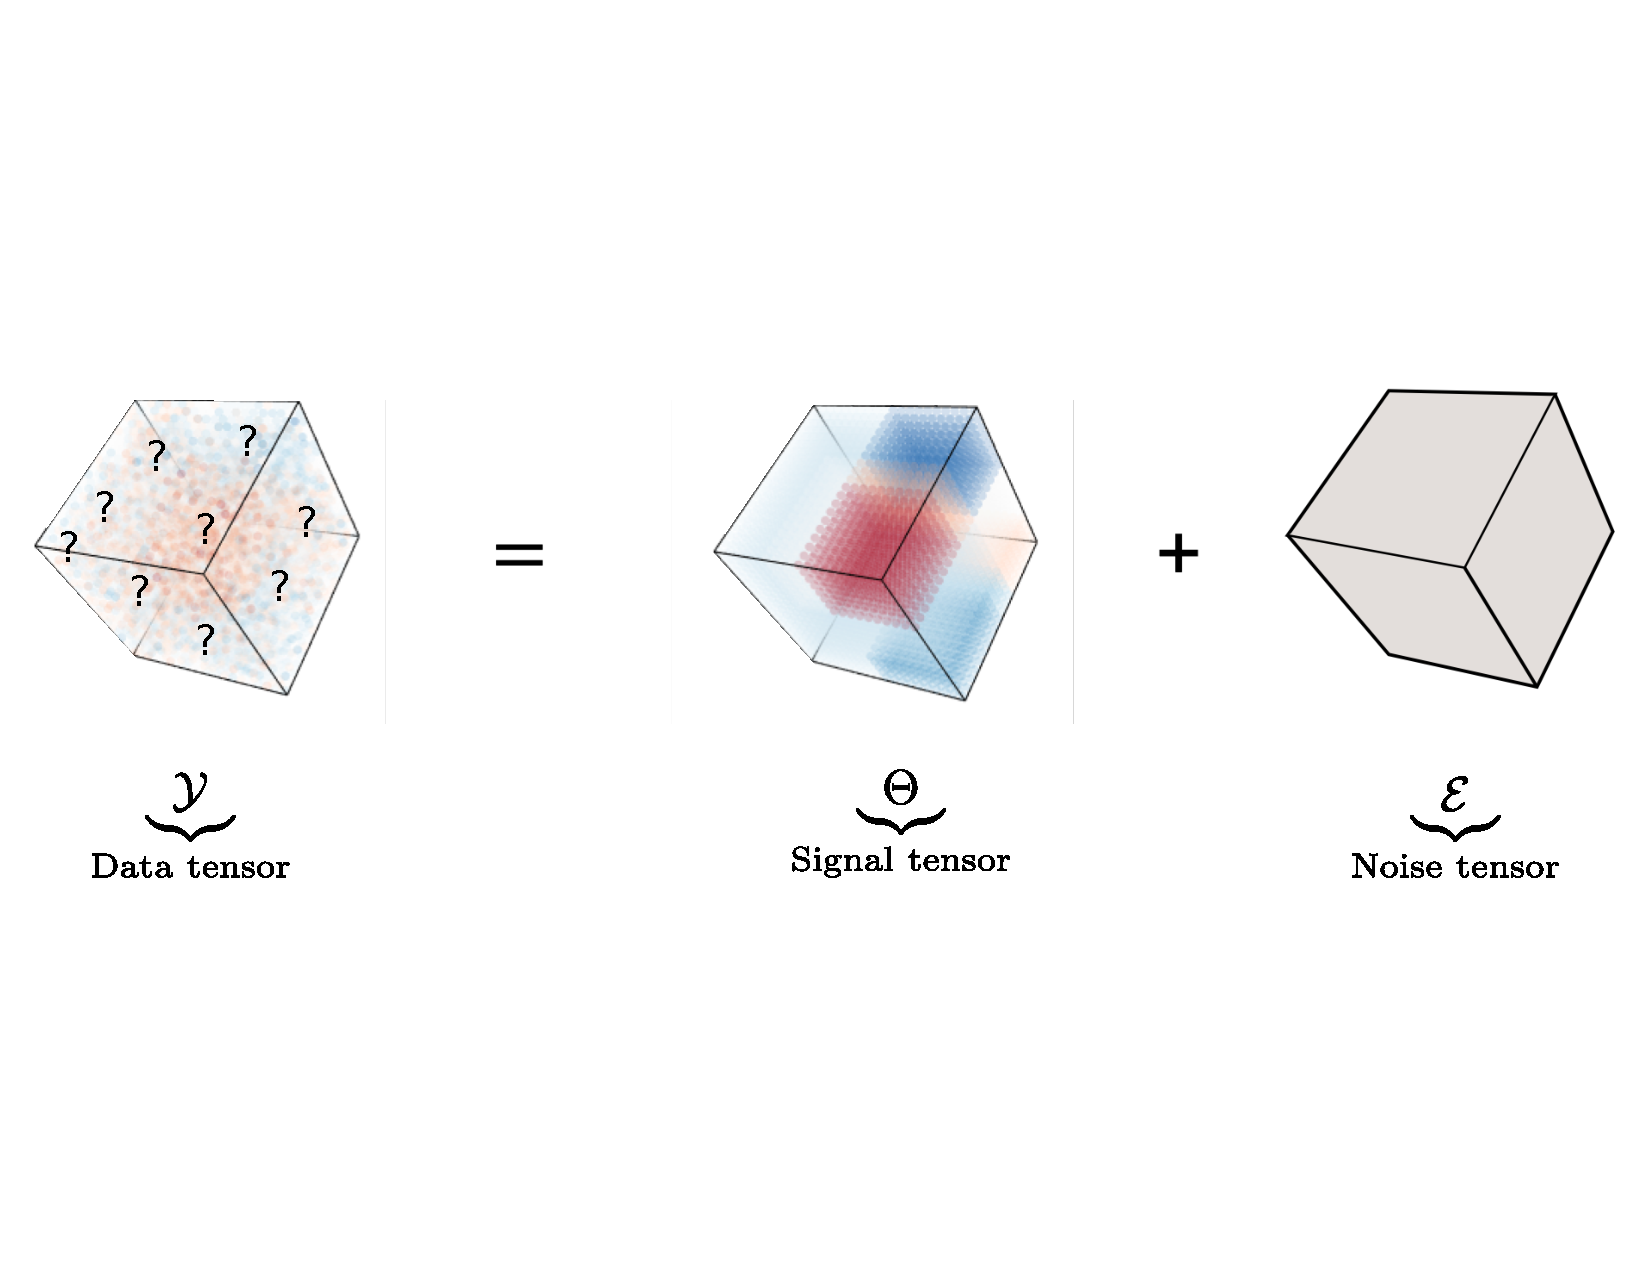
\includegraphics[width =\textwidth]{signalnoise.pdf}
    \end{center}
    \onslide<2->{
    We focus on the two problems
    \begin{enumerate}
        \item {\color{red}Nonparametric tensor estimation}: How to estimate the signal tensor $\Theta$?
        \item {\color{red}Complexity of tensor completion}: How many observed tensor entries do we need?
    \end{enumerate}}
\end{frame}

\begin{frame}{Classical approach}
 \begin{itemize}
 \item Low rank models~\citep{jain2014provable,montanari2018spectral}.\\[.5cm]

    \begin{center}
    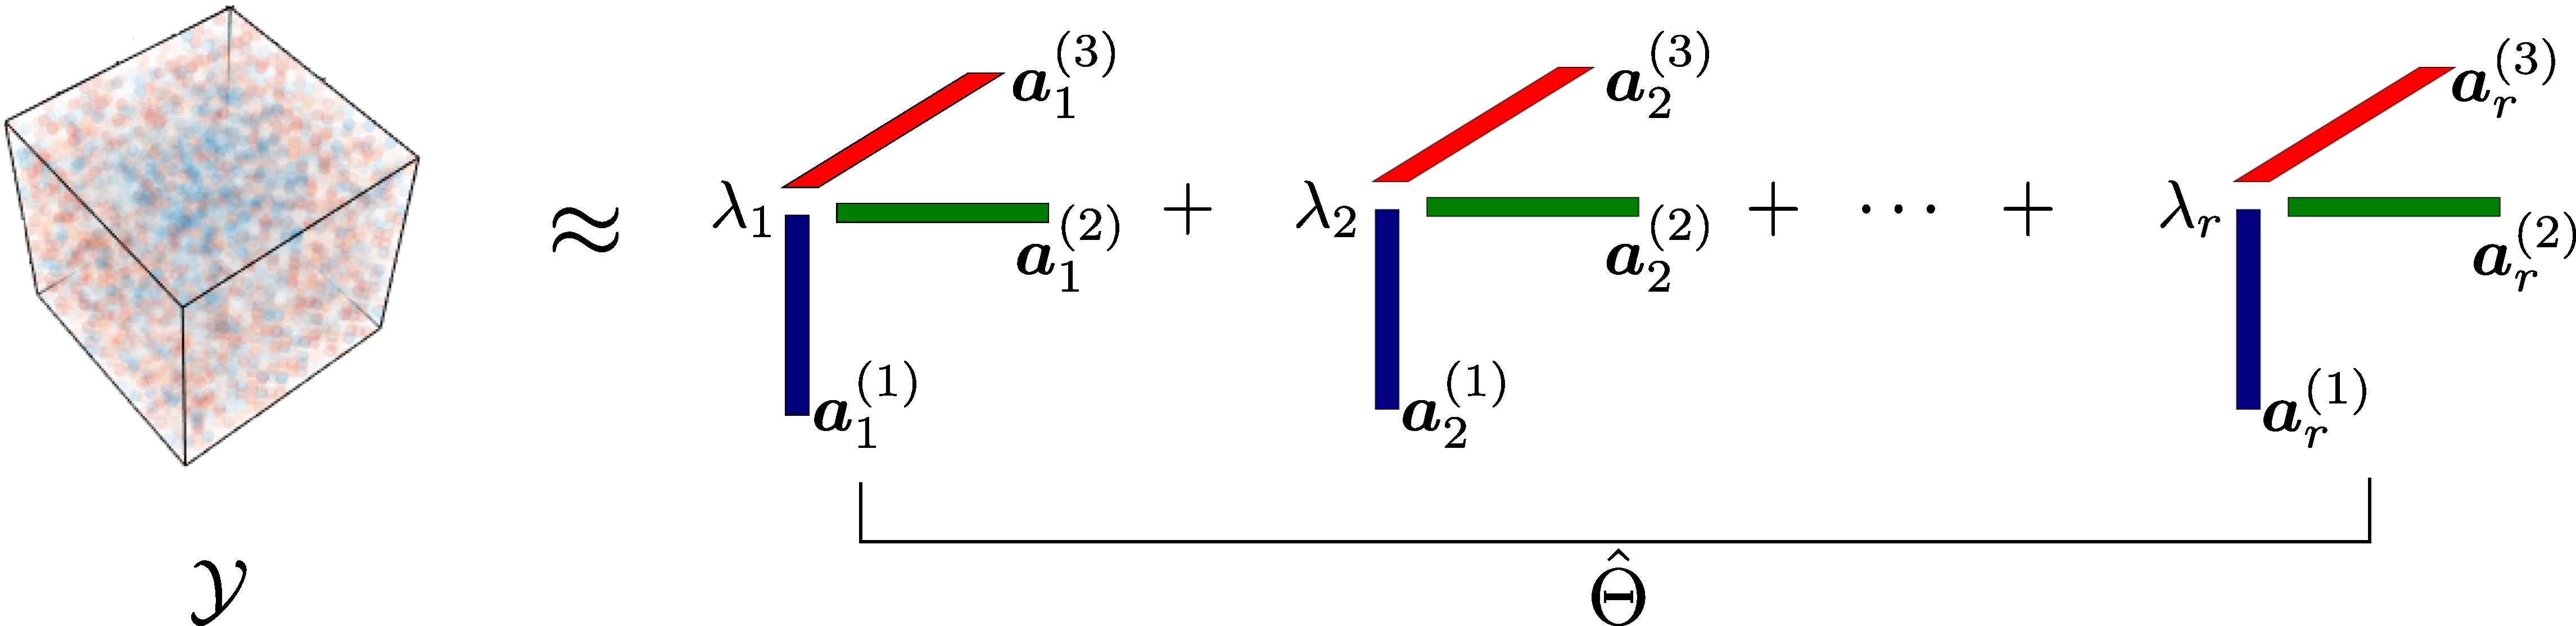
\includegraphics[width =\textwidth]{classic.pdf}
    \end{center}
\onslide<2->{
     \item There are two limitations of the model
     \begin{enumerate}
         \item The sensitivity to order-preserving transformation.
         \item Inadequacy for special structures.
     \end{enumerate}}
 \end{itemize}
\end{frame}

\begin{frame}{Classical approach}
 \begin{itemize}         
    \item The sensitivity to order-preserving transformation.
      \begin{columns}
\begin{column}{0.6\textwidth}
   \begin{center}
     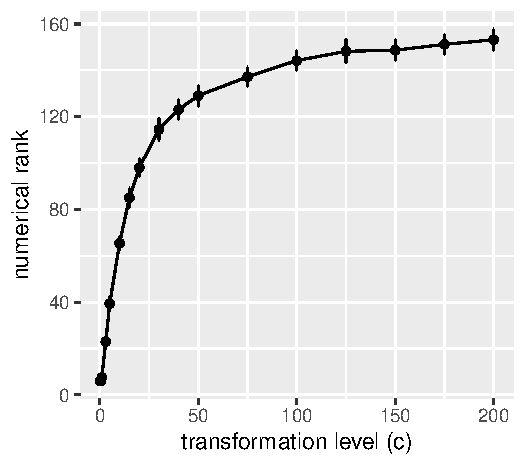
\includegraphics[width=0.5\textwidth]{example1.pdf}
     \end{center}
\end{column}
\begin{column}{0.5\textwidth} 
\begin{align}\Theta &= {1\over 1+\exp(-c\left(\mathcal{Z}\right))},\quad\text{ where }\\&\tZ = \bm a^{\otimes3}+ \bm b^{\otimes3}+ \bm c^{\otimes3}.\end{align}

\end{column}
\end{columns}
      
      \onslide<2->{
    \item Inadequacy for special structures.
      \begin{columns}
\begin{column}{0.7\textwidth}
   \begin{center}
     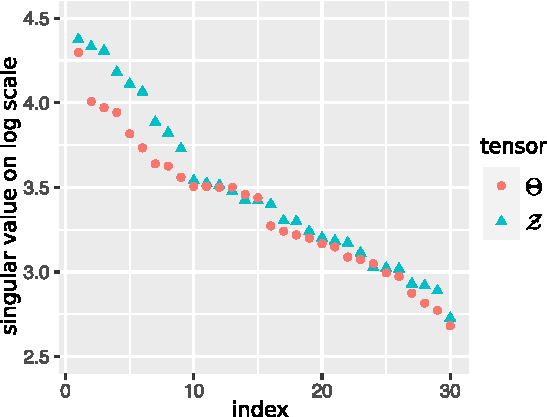
\includegraphics[width=0.5\textwidth]{example2.pdf}
     \end{center}
\end{column}
\begin{column}{0.5\textwidth}  %%<--- here
\begin{align}\Theta &= \log(1+\mathcal{Z}),\quad\text{ where }\\&\mathcal{Z}(i,j,k) = \frac{1}{d}\max(i,j,k). \text{ }\hspace{1cm} \end{align}

\end{column}
\end{columns}
    
  }
 \end{itemize}
\end{frame}

\begin{frame}{Motivational toy example}
    \begin{center}
    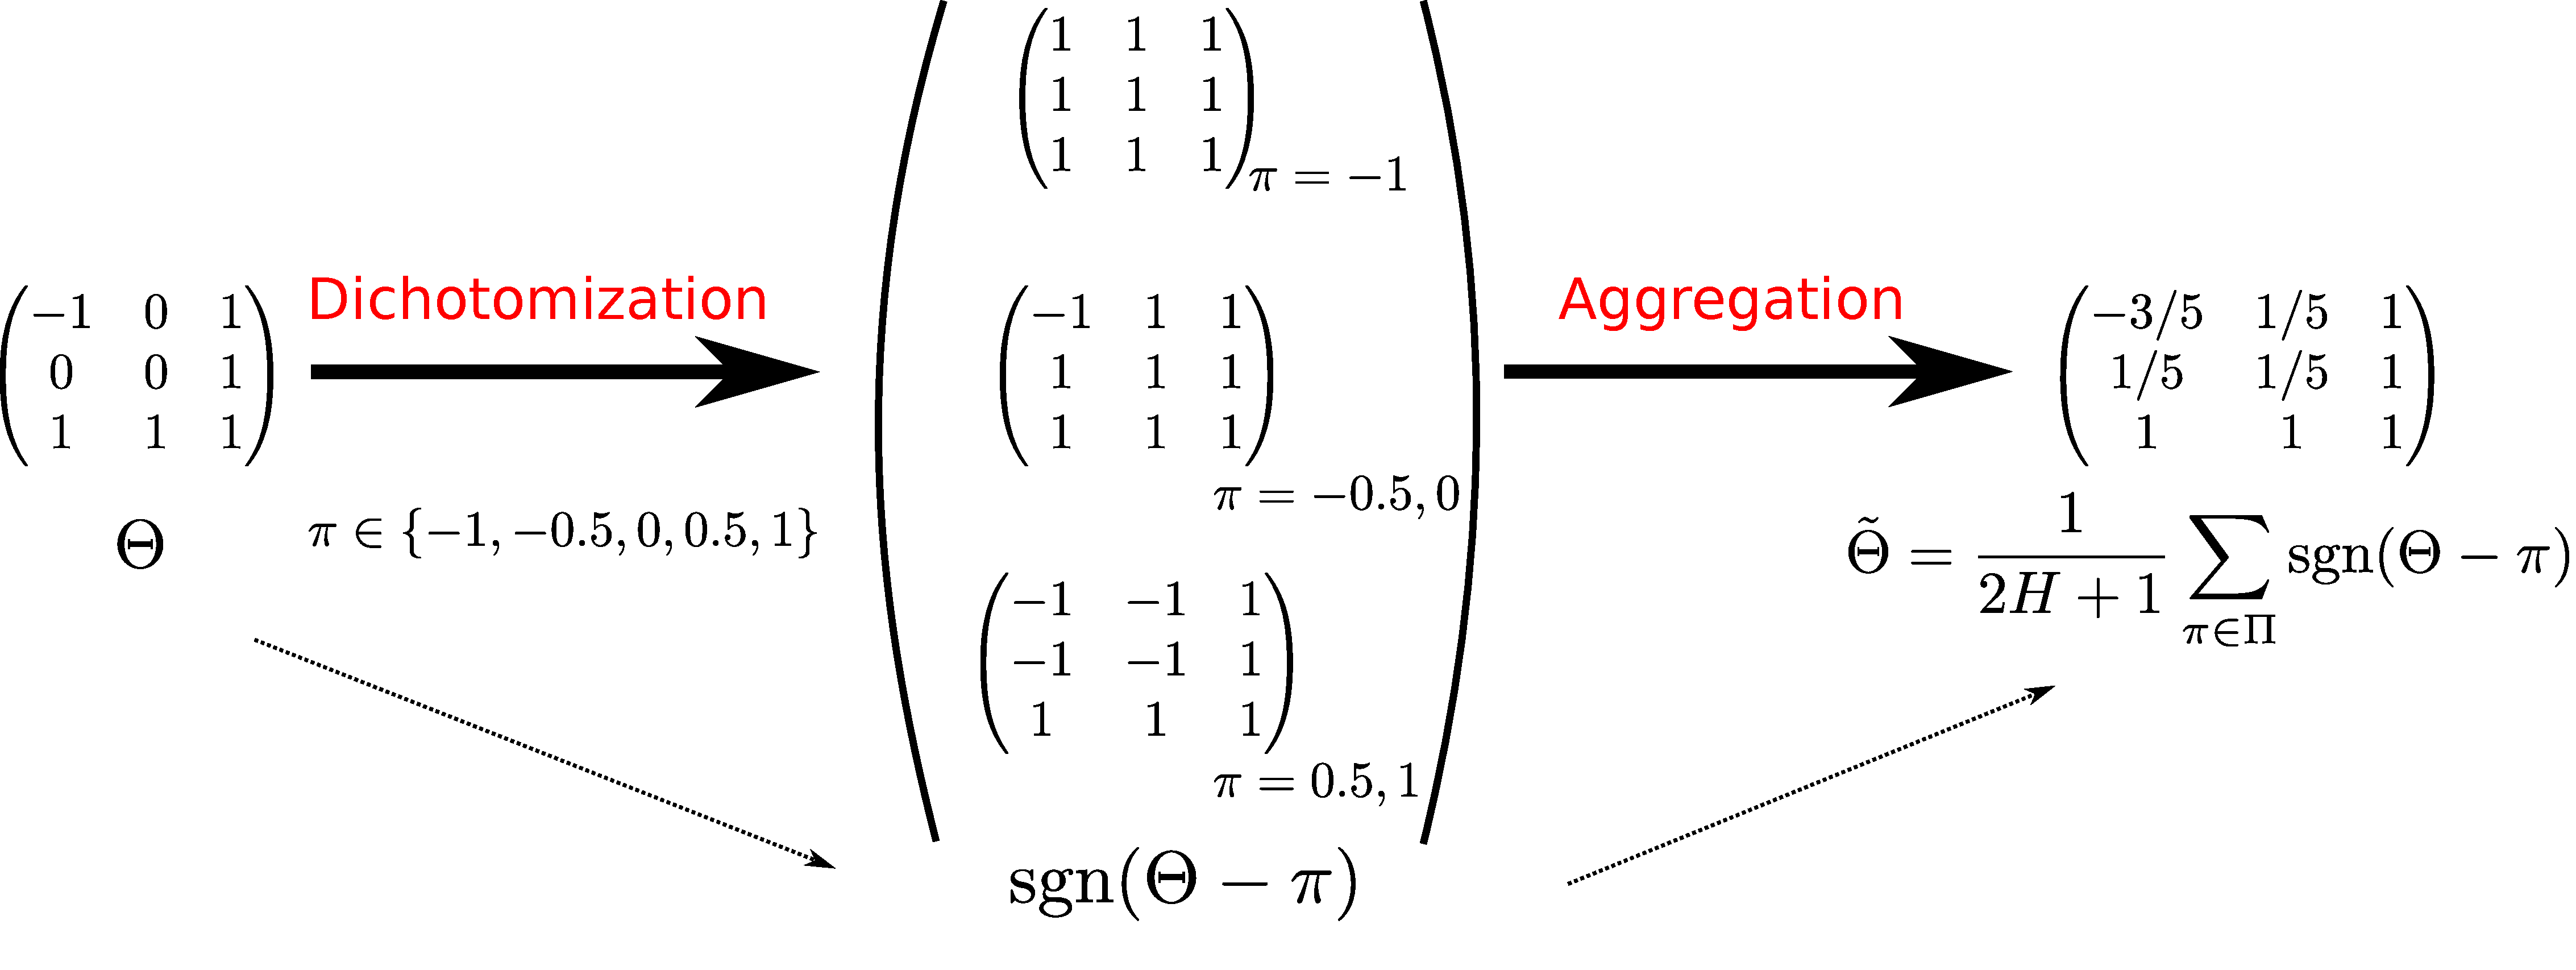
\includegraphics[width =\textwidth]{toyexample.pdf}
    \end{center}
{\footnotesize where $\text{sgn}(x) = \begin{cases}1,&\text{ if } x\geq 0,\\-1 &\text{ otherwise.}\end{cases}$}
\onslide<2->{
    \begin{itemize}
    \item We do not use magnitude of the signal tensor but {\color{red}sign representation}.
     \item With a series of sign tensors, we can successfully preserve all information in the original signals.
    \end{itemize}
 }
\end{frame}



\begin{frame}{Sign rank}
\begin{itemize}
    \item  Two tensors are sign equivalent denoted as $\Theta \simeq \Theta'$ if $\text{sgn}(\Theta) = \text{sgn}(\Theta')$.

    \item Sign rank is defined as
    \begin{align}
    \rlap{\textcolor{blue!10}{\rule[-\dp\strutbox]{235pt}{\baselineskip}}}\,\text{srank}(\Theta) = \min\{\text{rank}(\Theta')\colon \Theta'\simeq \Theta, \Theta'\in\mathbb{R}^{d_1\times\cdots\times d_K}\}.
    \end{align}
    \onslide<2->{
 \begin{center}
    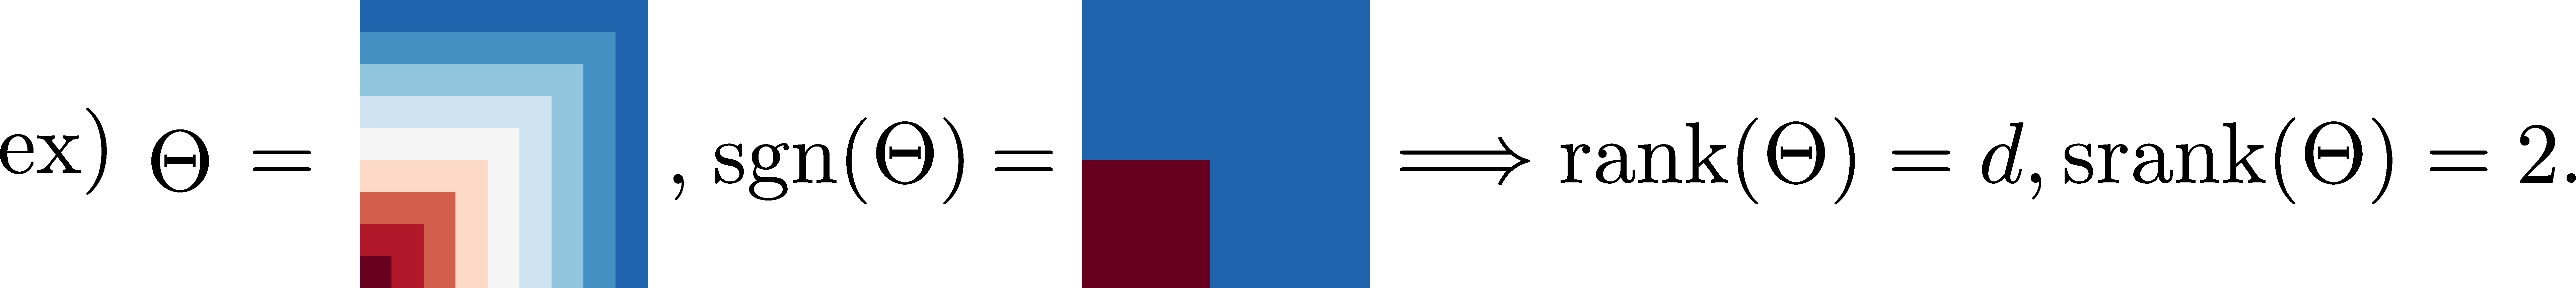
\includegraphics[width =\textwidth]{signrank.pdf}
    \end{center}}
    \onslide<3->{
\item In fact, for any strictly monotonic function $g\colon\mathbb{R}\rightarrow \mathbb{R}$ with $g(0) = 0$,
\[\rlap{\textcolor{blue!10}{\rule[-\dp\strutbox]{105pt}{\baselineskip}}}\,\text{srank}(\Theta)\leq \text{rank}(g(\Theta)).\]}
\end{itemize}


\end{frame}

\begin{frame}{Sign representable tensors}
    \begin{block}{Sign representable tensors} A tensor $\Theta$ is called $r$-sign representable if the tensor $(\Theta-\pi)$ has sign rank bounded by $r$ for all $\pi\in[-1,1].$ The collection $\{\text{sgn}(\Theta-\pi)\colon \pi\in[-1,1]\}$ is called the sign tensor series.
    \end{block}
     ex1) $\Theta = \begin{pmatrix}-1&0&1\\0&0&1\\1&1&1\end{pmatrix}$ is 2-sign representable.
       \\[.1cm] ex2) $\Theta(i_1,\ldots,i_K) = \log(1+\max(i_1,\ldots,i_K))$ is 2-sign representable.
       \\[.1cm] ex3) $\Theta$ such that $\text{rank}(\Theta)\leq r$, is $(r+1)$-sign representable.
    \begin{itemize} 
    \onslide<2->{
       \item Instead of the classical low rank assumption, we assume
       \begin{align}
         \rlap{\textcolor{blue!10}{\rule[-\dp\strutbox]{250pt}{\baselineskip}}}\,  \Theta\in\caliP(r):=\{\Theta\colon\text{srank}(\Theta-\pi)\leq r \text{ for all } \pi\in[-1,1]\}.
       \end{align}}
      \end{itemize}
\end{frame}



\begin{frame}{Our new approach}
    \begin{center}
    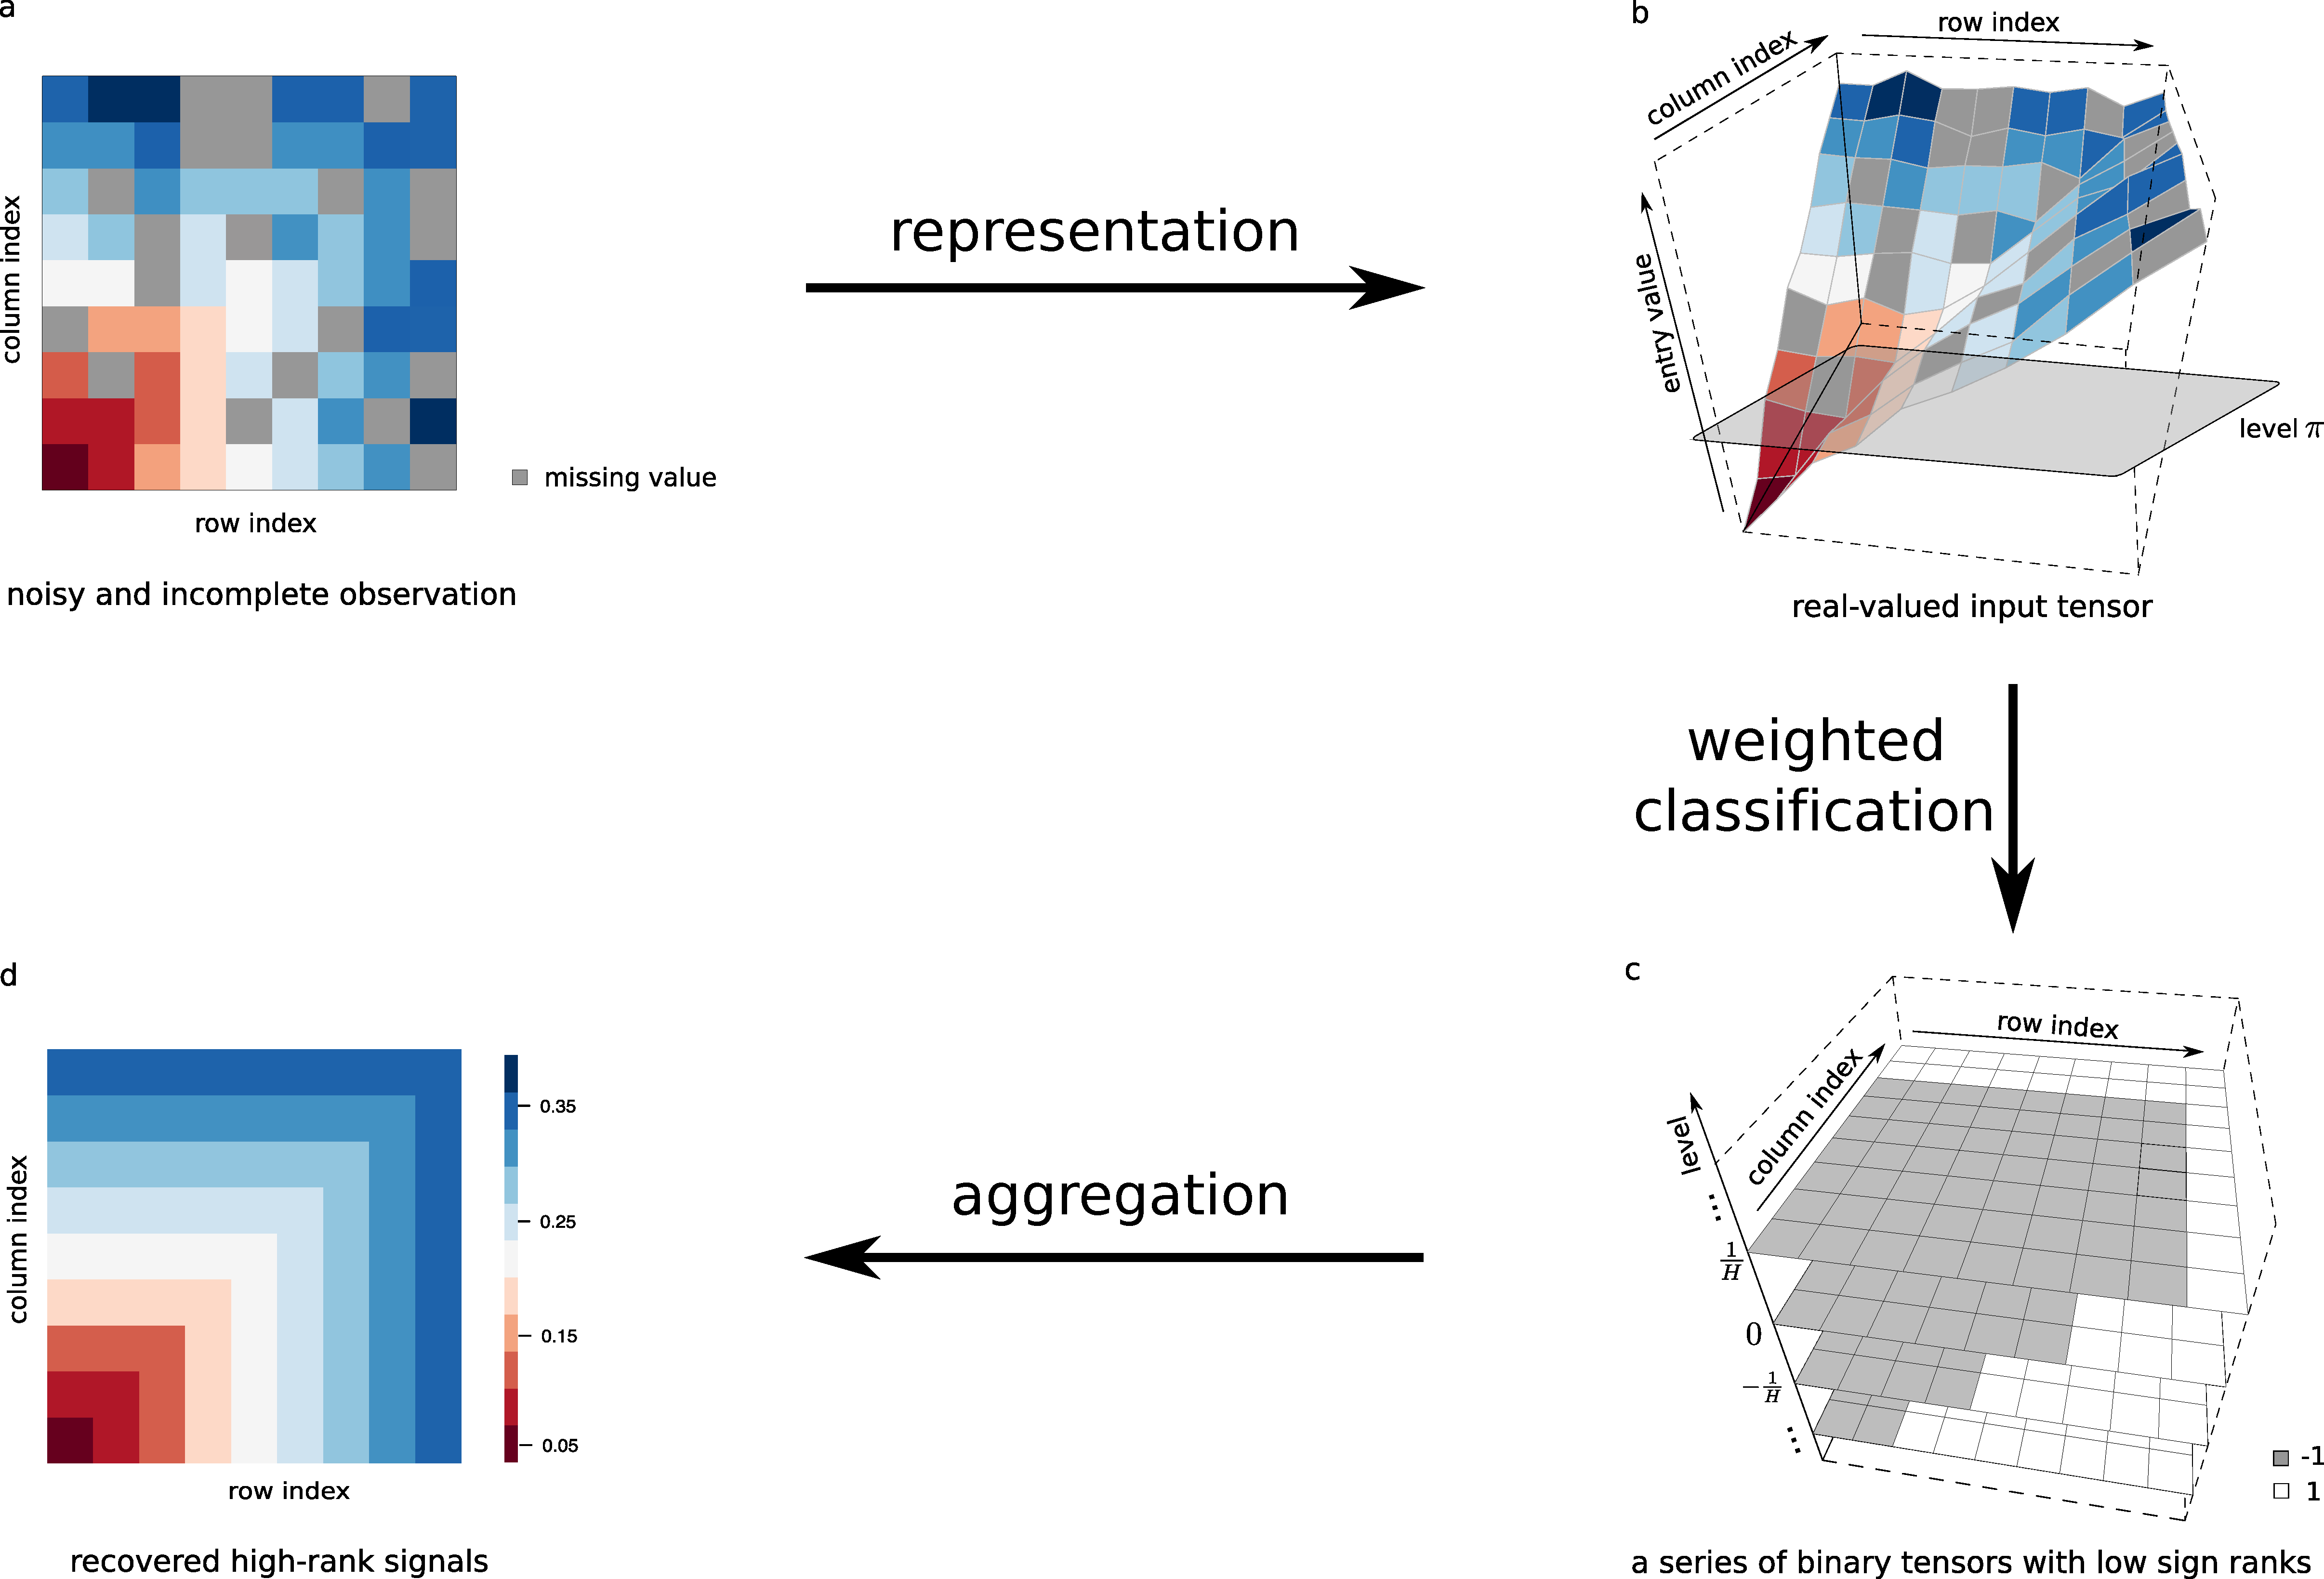
\includegraphics[width =\textwidth]{mainidea.pdf}
    \end{center}
 
\end{frame}

\begin{frame}{Our new approach: representation}
  \begin{center}
    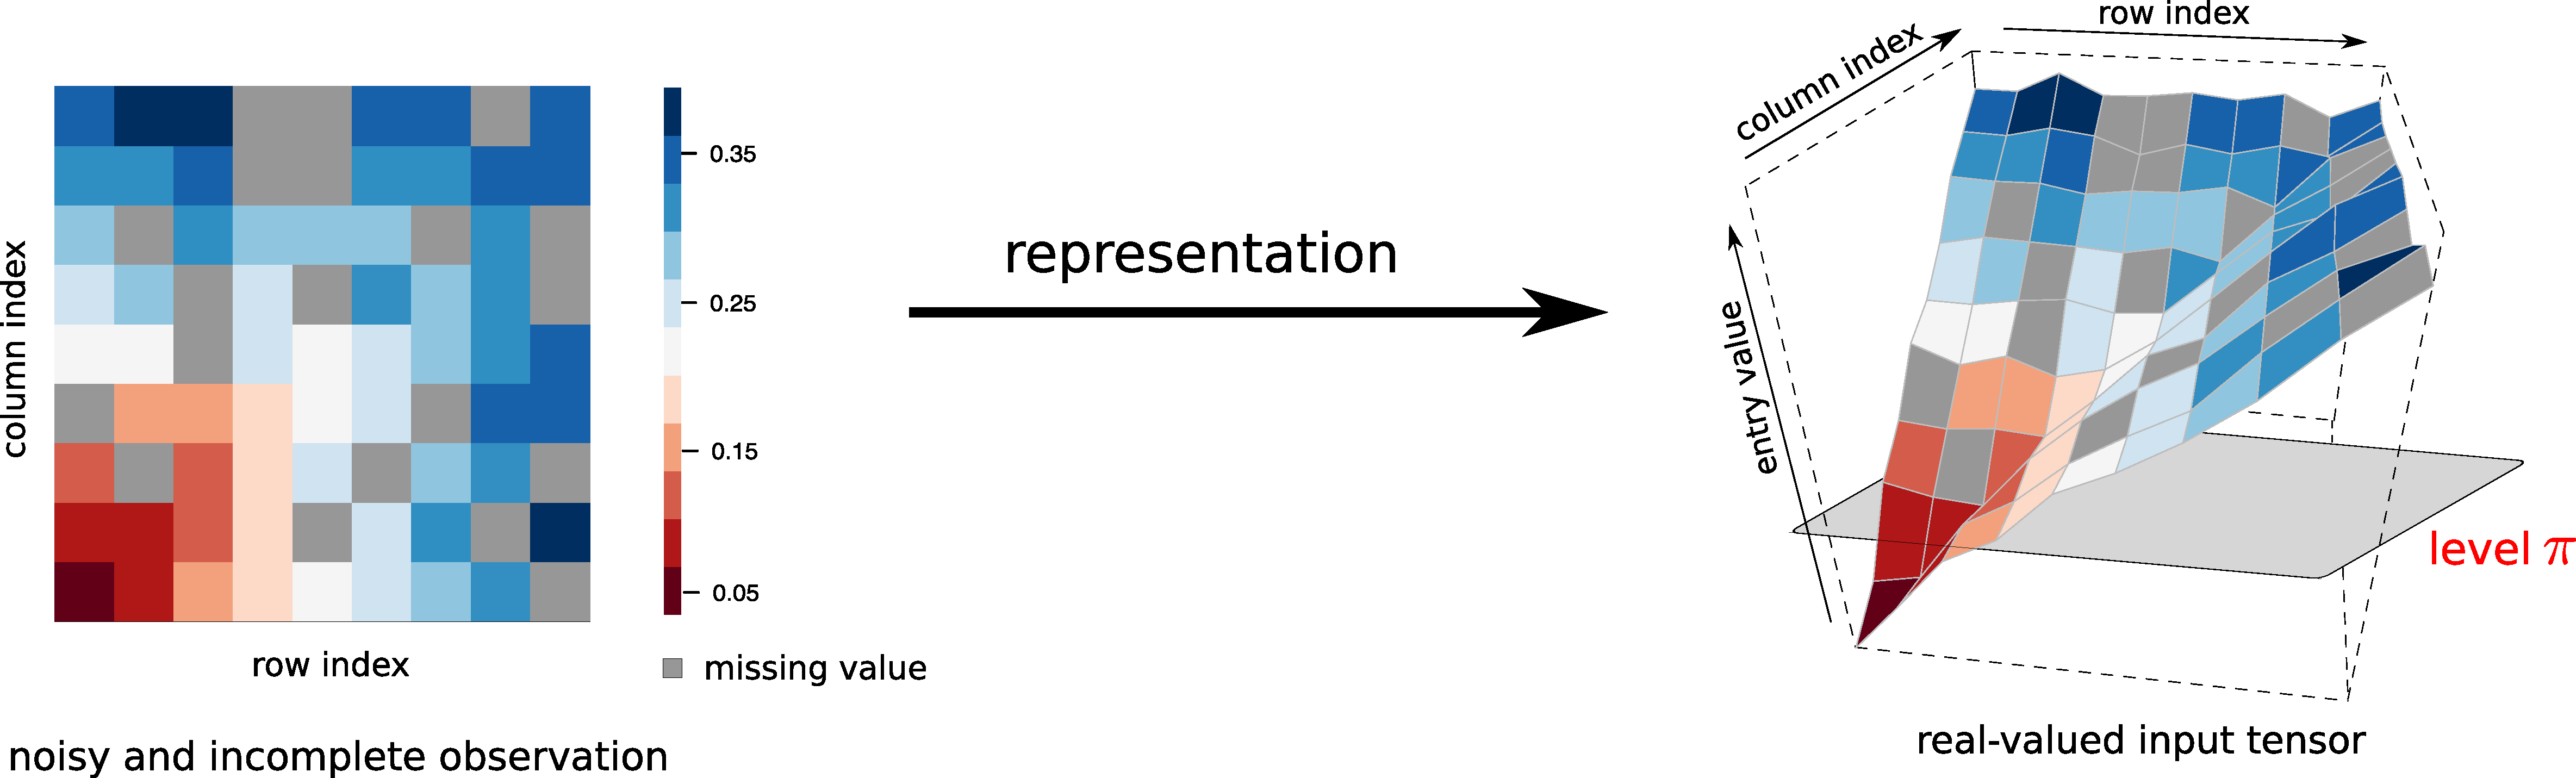
\includegraphics[width =\textwidth]{representation.pdf}
    \end{center}
\begin{itemize}
    \item We are given the observed tensor $\tY_\Omega\in[-1,1]^{d_1\times \cdots\times d_K}$ with observed index set $\Omega\in[d_1]\times\cdots\times[d_K]$.
    \item We obtain sign tensor series \[\{\text{sgn}(\tY_\Omega-\pi)\}_{\pi\in\tH},\quad \text{ where } \tH= \{-1,\ldots,-1/H,0,1/H,\ldots,1\}.\]
\end{itemize}
    
\end{frame}
\begin{frame}{Our new approach: weighted classification}
    \begin{center}
    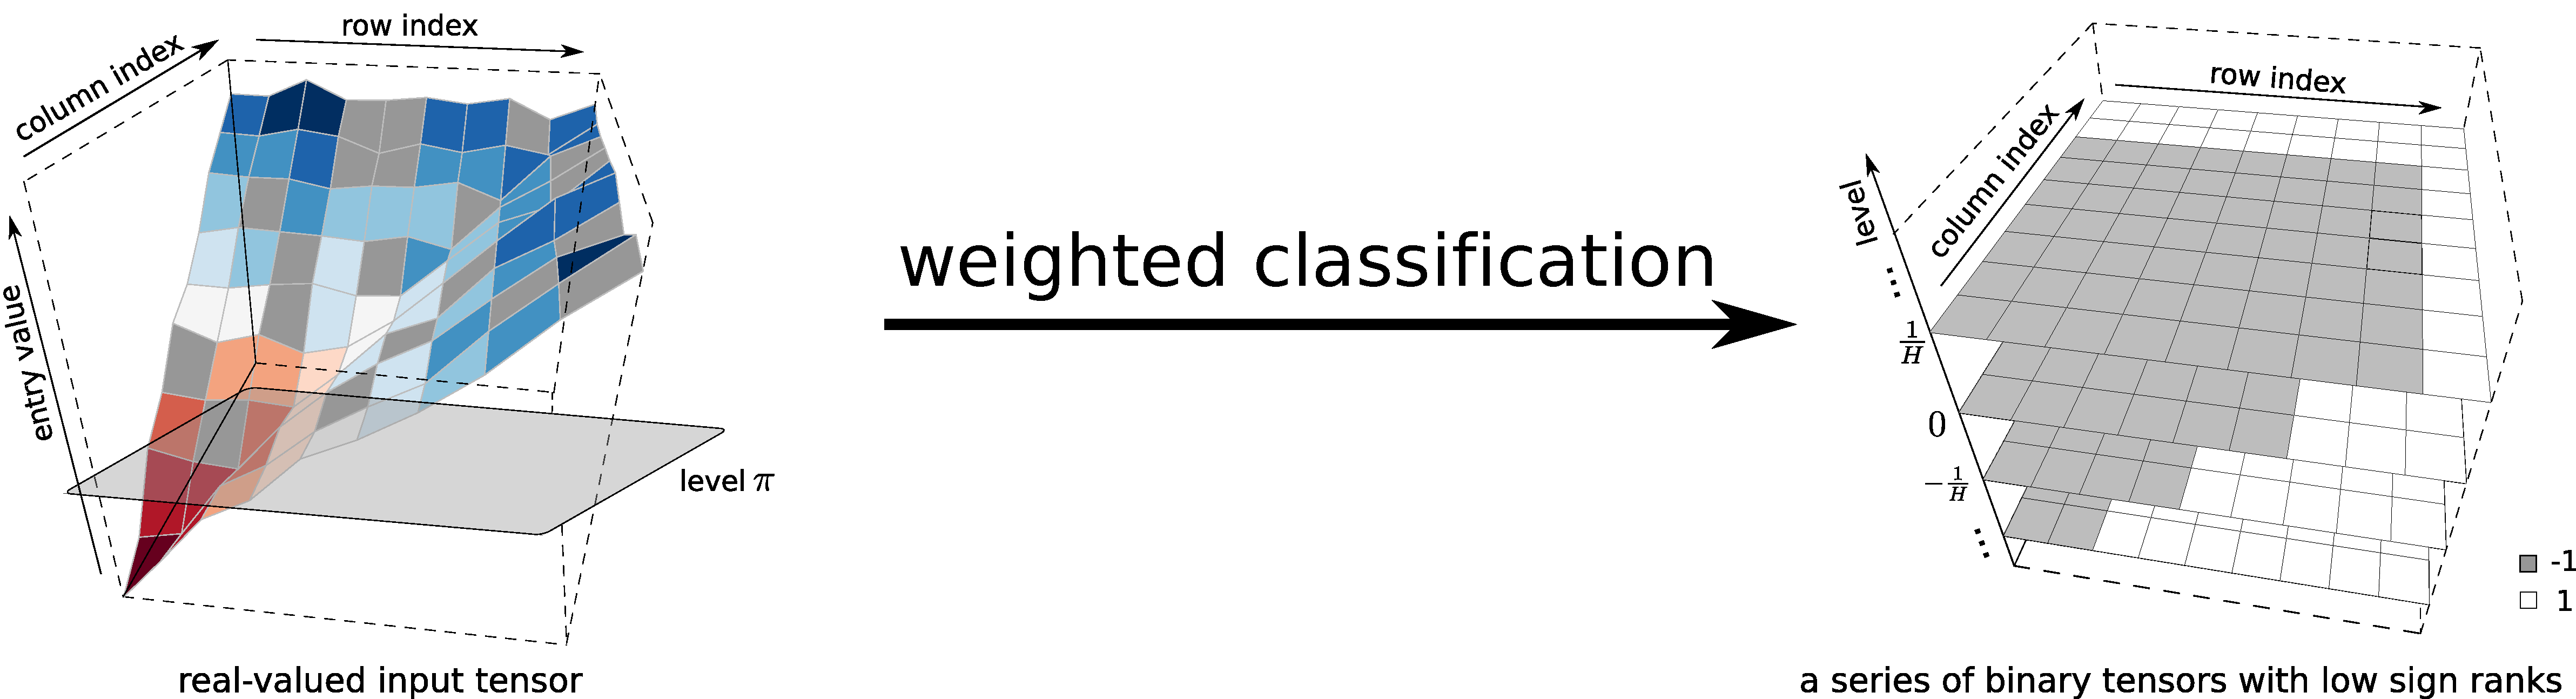
\includegraphics[width =\textwidth]{weightedclassification.pdf}
    \end{center}
    \begin{itemize}
    \item We estimate $\text{sgn}(\Theta-\pi)$ through $\text{sgn}(\tY_\Omega-\pi)$ via weighted classification.
    \item Objective function of weighted classification is
    \begin{align}
    L(\tZ,\tY_\Omega-\pi) = \frac{1}{|\Omega|}\sum_{\pi\in\Omega}\underbrace{|\tY(\omega)-\pi|}_{\text{weight}}\times\underbrace{ |\text{sgn}(\tZ(\omega))-\text{sgn}(\tY(\omega)-\pi)|}_{\text{classification loss}}
    \end{align}
    \end{itemize}
\end{frame}


\begin{frame}{Our new approach: weighted classification}
\begin{block}{$\alpha$ smoothness}
For fixed $\pi$, we call $\Theta$ is $\alpha$ smooth if there exist $\alpha = \alpha(\pi)>0,c = c(\pi)>0$, such that 
\begin{align}
    \sup_{0\leq t<\rho(\pi,\tN)}{\mathbb{P}_{\omega\sim\pi}[|\Theta(\omega)-\pi|\leq t]\over t^\alpha}\leq c,
\end{align}
where $\rho(\pi,\tN) = \min_{\pi'\in\tN}|\pi-\pi'|$ and $\tN = \{\pi\colon\mathbb{P}(\Theta(\omega) = \pi)\neq 0\}$.
If constants $\alpha$ and $c$ are independent of $\pi$, we call $\Theta$ is $\alpha$-globally smooth.
\end{block}
 \begin{center}
 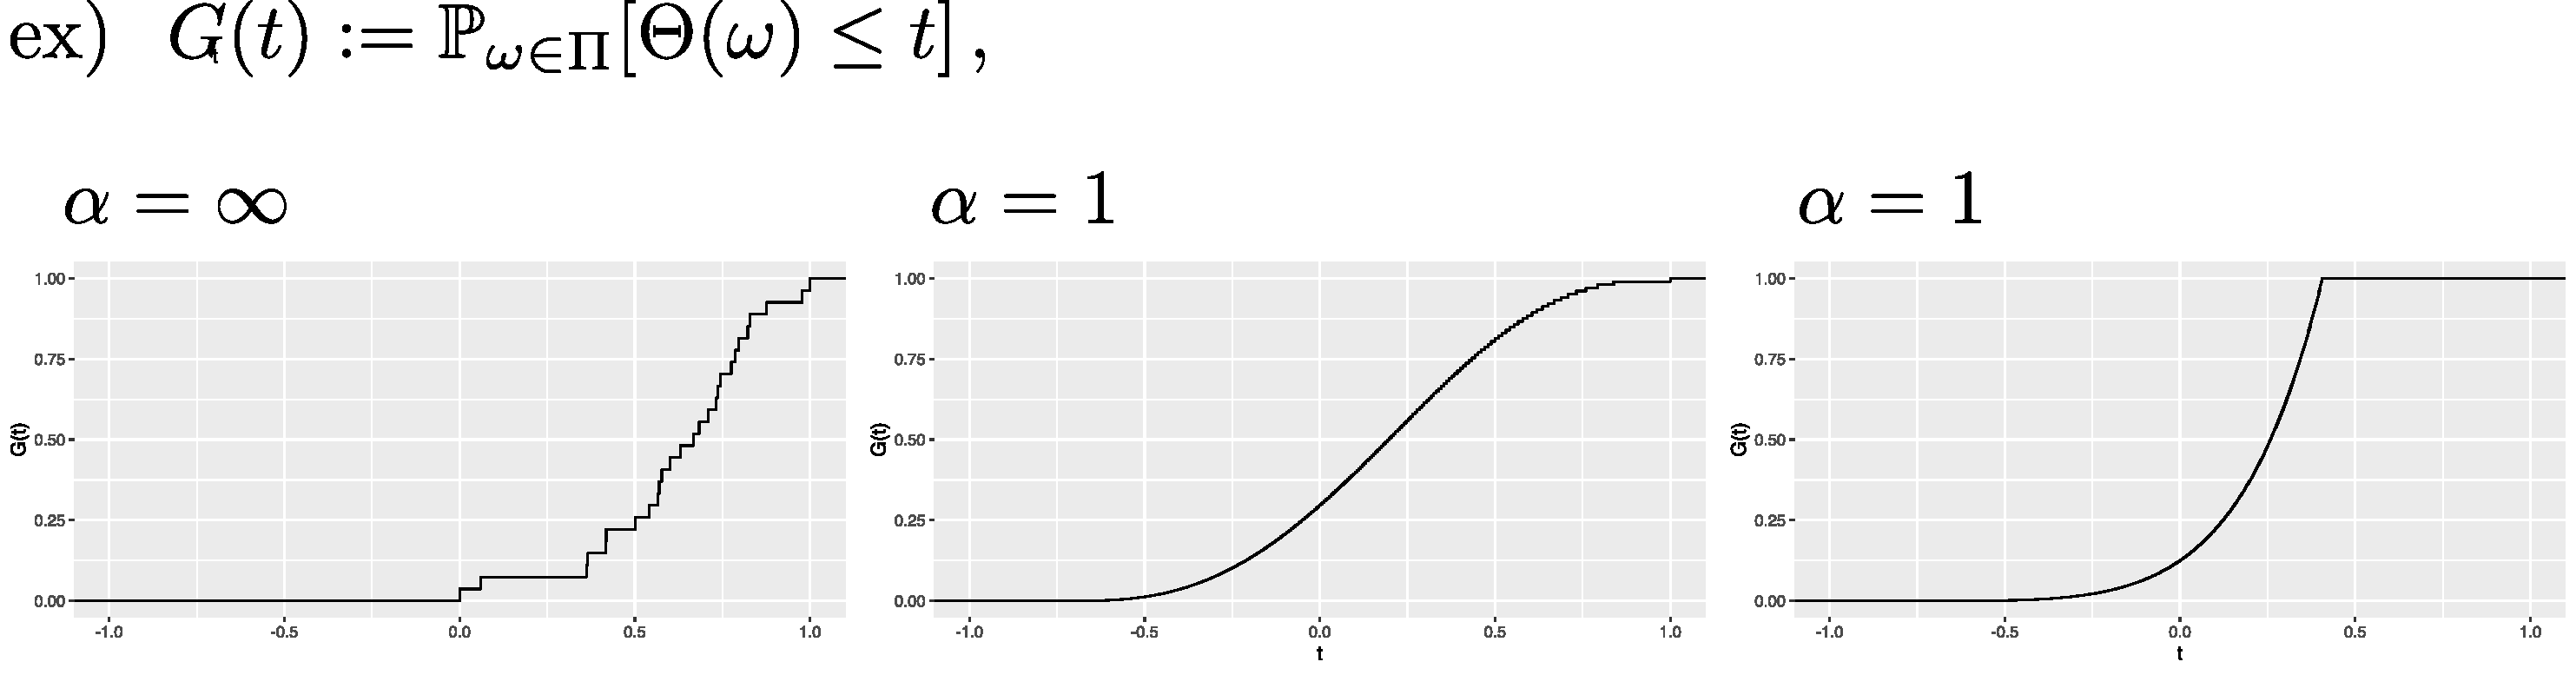
\includegraphics[width = \textwidth]{cdf.pdf}
 \end{center}
\end{frame}


\begin{frame}{Our new approach: weighed classification}
 \begin{center}
 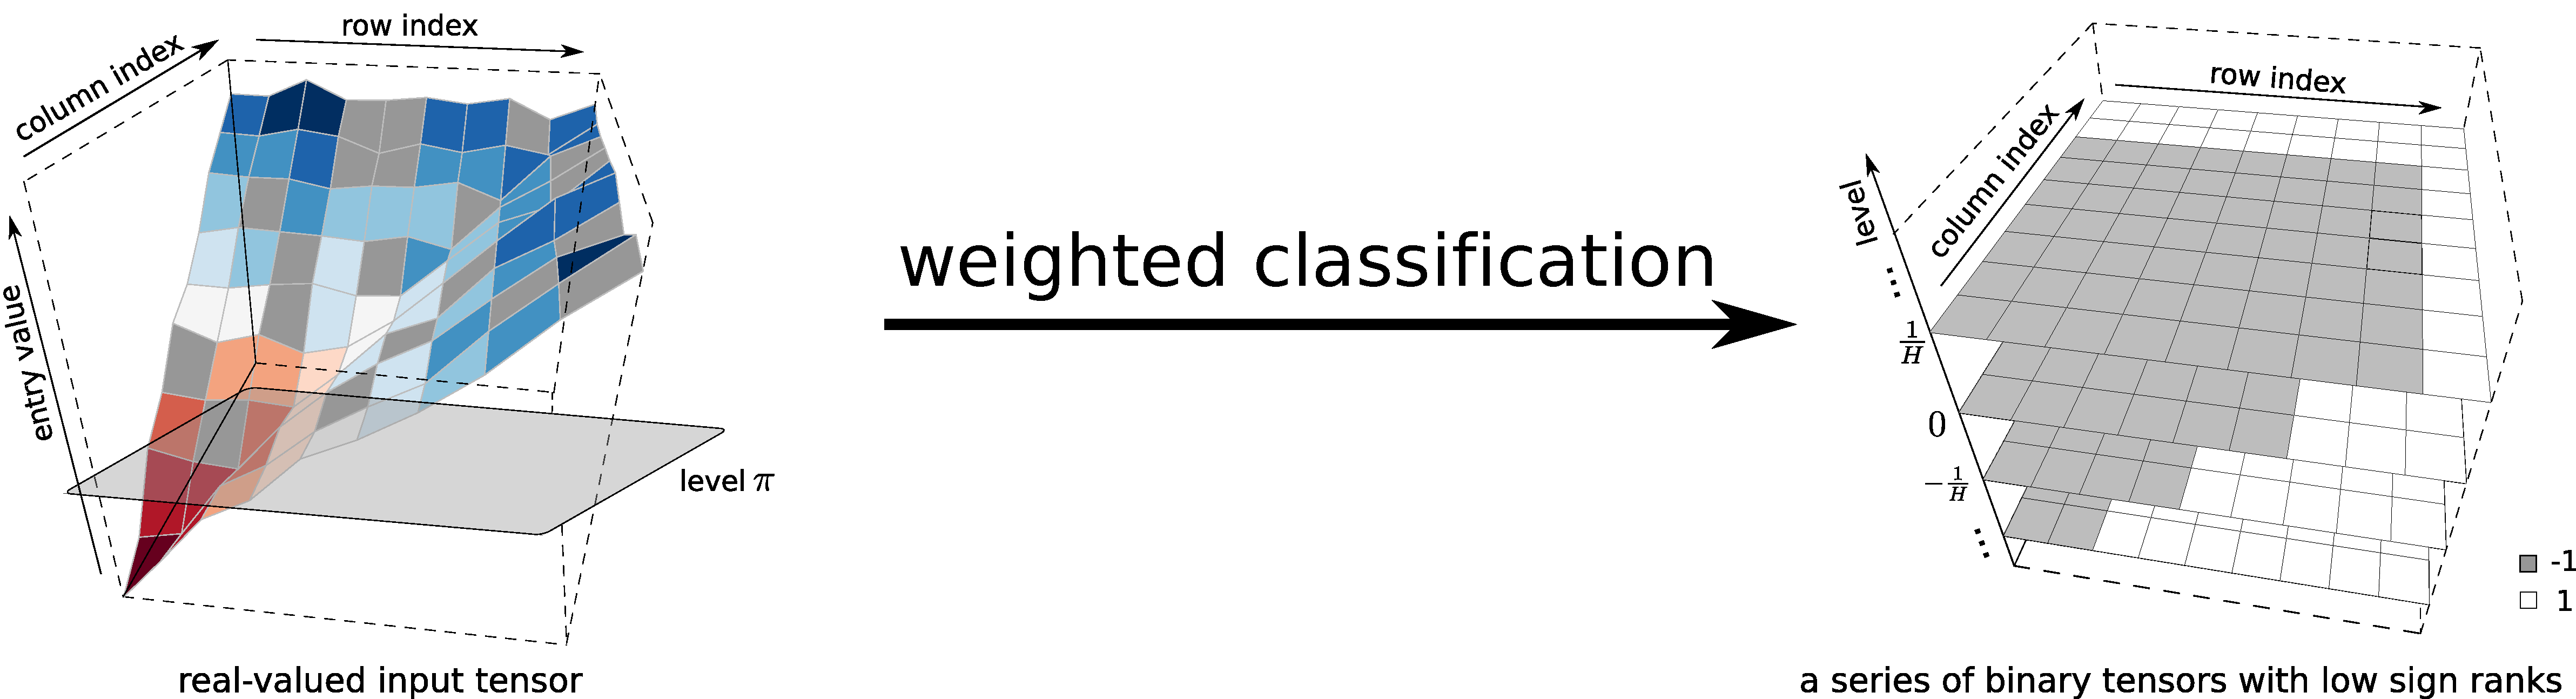
\includegraphics[width = \textwidth]{weightedclassification.pdf}
 \end{center}
   \begin{itemize}
    \item If $\Theta$ is $\alpha$ smooth ($\alpha>0$), we have {\color{red}an unique optimizer}  such that\\[.1cm]
       $\hspace{2cm}\text{sgn}(\Theta-\pi) = \argmin\limits_{\tZ\colon \text{rank}(\tZ)\leq r} \mathbb{E}_{\tY_\Omega}L(\tZ,\tY_\Omega-\pi)$.\vspace*{.1cm}

    \item So we obtain a series of optimizers $\{\hat \tZ_\pi\}_{\pi\in\tH}$ as
    \begin{align}
        \hat \tZ_\pi = \argmin_{\tZ\colon \text{rank}(\tZ)\leq r}L(\tZ,\tY_\Omega-\pi).
    \end{align}
    \end{itemize}
\end{frame}

\begin{frame}{Our new approach: aggregation}
    \begin{center}
    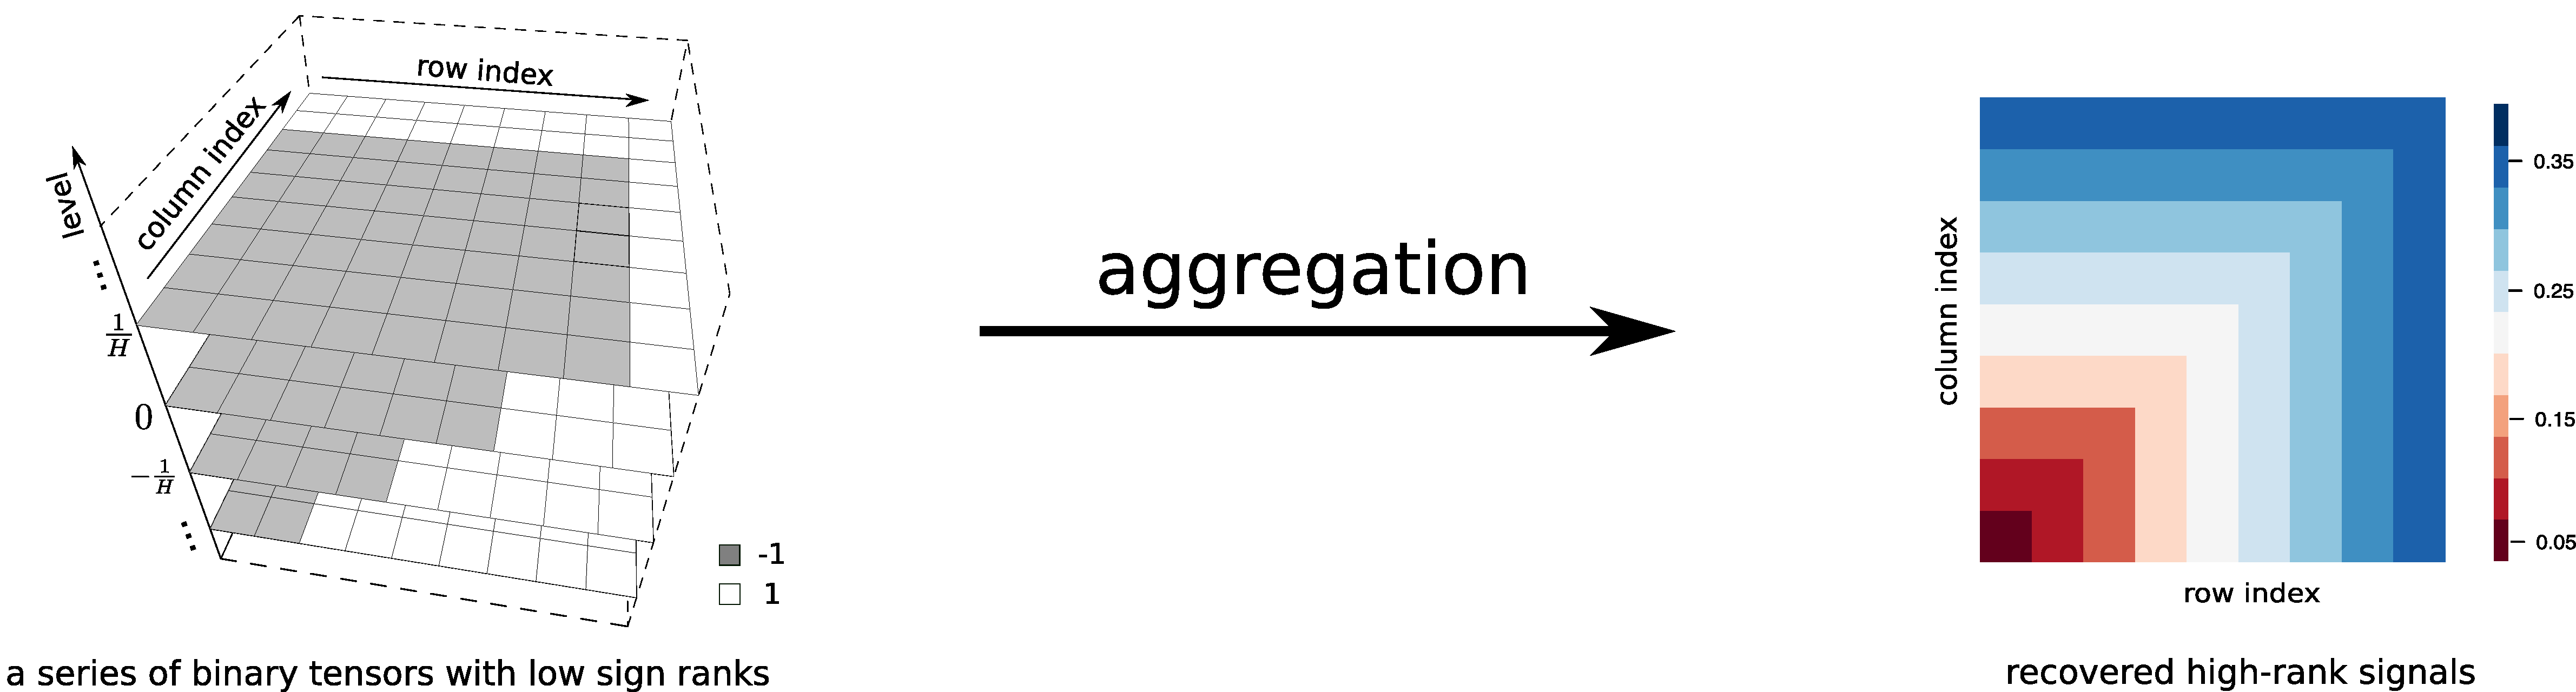
\includegraphics[width =\textwidth]{aggregation.pdf}
    \end{center}
    \begin{itemize}
    \item From a series of optimizers $\{\hat\tZ_\pi\}_{\pi\in\tH}$ in the weighted classification, we propose the tensr estimate 
    \begin{align}
        \hat\Theta = {1\over 2H+1}\sum_{\pi\in\tH}\text{sgn}\hat \tZ_\pi.
    \end{align}
    \end{itemize}
\end{frame}


\begin{frame}{Theoretical results: sign tensor estimation error}
\begin{itemize}
\item For two tensor $\Theta_1,\Theta_2$, define $\textup{MAE}(\Theta_1,\Theta_2) = \mathbb{E}_{\omega\in\Pi}|\Theta_1(\omega)-\Theta_2(\omega)|.$
\end{itemize}
    \begin{block}{Sign tensor estimation for fixed $\pi$ (L. and Wang, 2021)}
    Suppose $\Theta\in\caliP(r)$ and  $\Theta(\omega)$ is $\alpha$ smooth for fixed $\pi$. $d_{\max}=\max_{k\in[K]} d_k$. Then, with very high probability over $\tY_\Omega$, 
\begin{align}
\textup{MAE}(\text{sgn}\hat \tZ_\pi, \text{sgn}(\Theta-\pi)) \lesssim  \left({d_{\max} r\over |\Omega|}\right)^{\alpha\over \alpha+2}.
\end{align}
    \end{block}
\end{frame}

\begin{frame}{Theoretical results: tensor estimation error}
    \begin{block}{Tensor estimation error (L. and Wang 2021)}
    Suppose $\Theta\in\caliP(r)$ and  $\Theta(\omega)$ is $\alpha$-globally smooth. Then, with very high probability over $\tY_\Omega$, 
    \begin{equation}\label{eq:bound2}
\textup{MAE}(\hat \Theta, \Theta)\lesssim \left({d_{\max} r \over |\Omega|}\right)^{\alpha\over\alpha+2}+{1\over H}+{Hd_{\max} r \over |\Omega|}.
\end{equation}
In particular, setting $\scriptstyle H\asymp \left( |\Omega|\over d_{\max}r\right)^{1/2}$ yields the error bound
\begin{equation}\label{eq:real}
\textup{MAE}(\hat \Theta, \Theta)\lesssim \left(d_{\max}r \over |\Omega|\right)^{{\alpha \over \alpha+2} \vee {1\over 2}}.
\end{equation}
    \end{block}
    \onslide<2->{
    \begin{itemize}
        \item Tensor estimation is generally no better than sign tensor estimation.
        \item Sample complexity: \[\text{MAE}(\hat\Theta,\Theta)\rightarrow 0, \text{ as } {|\Omega|\over d_{\max}r}\rightarrow\infty.\]
    \end{itemize}}
\end{frame}


\begin{frame}{Simulations}
    \begin{center}
    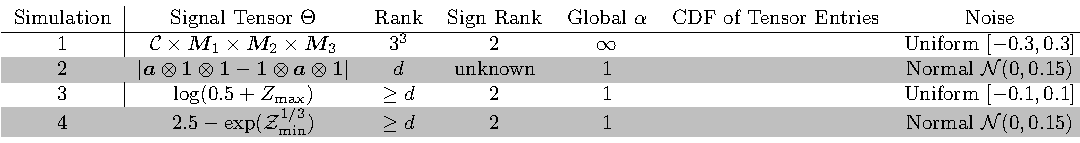
\includegraphics[width = \textwidth]{simulation.pdf}
    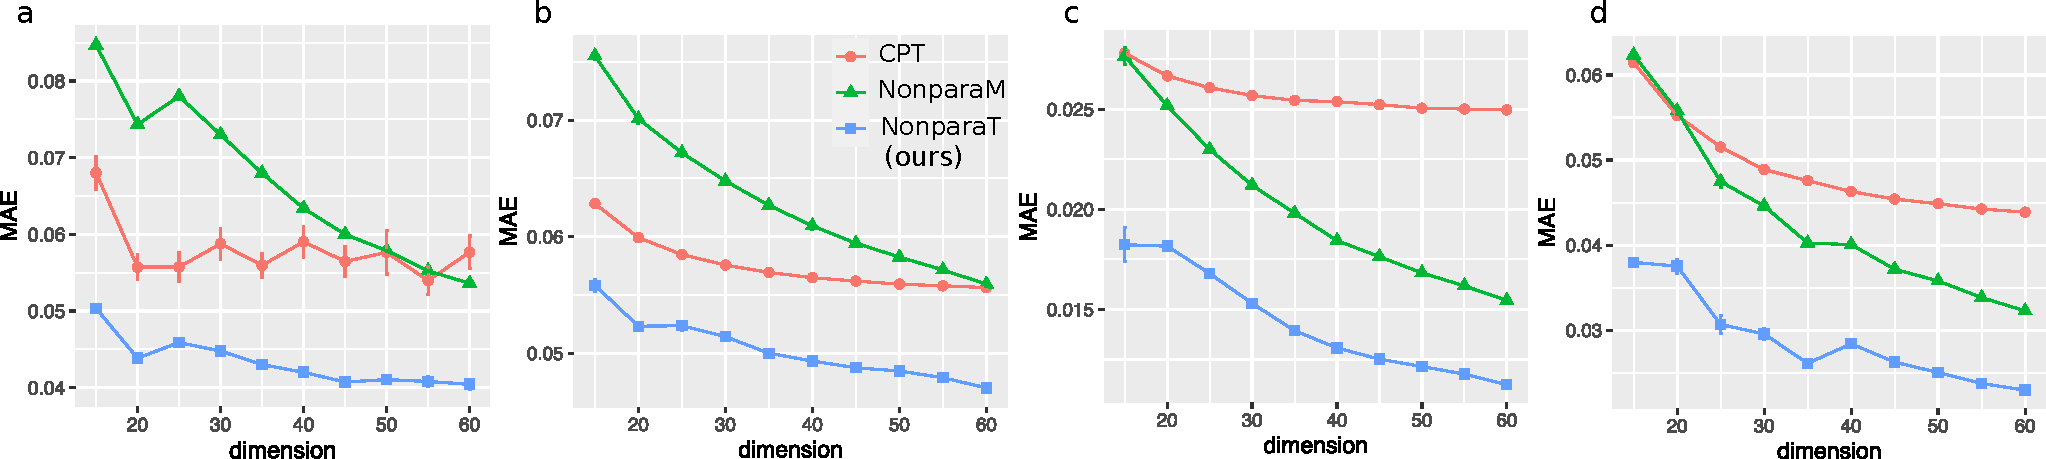
\includegraphics[width =\textwidth]{fig1-4v2.pdf}
    \end{center}
    \begin{itemize}
    \item {\bf NonPraT}: Our nonparametric tensor method, {\bf CPT}: low rank tensor CP decomposition, {\bf NonPraraM}: the matrix version of our method.
    \item Estimation versus tensor dimension.
    \item Our method (NonparaT) achives the best performance.
    \end{itemize}
\end{frame}

\begin{frame}{Simulations}
    \begin{center}
    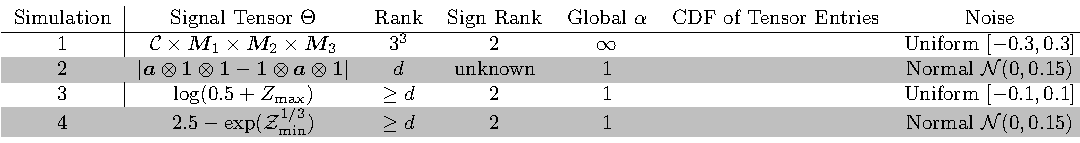
\includegraphics[width = \textwidth]{simulation.pdf}
    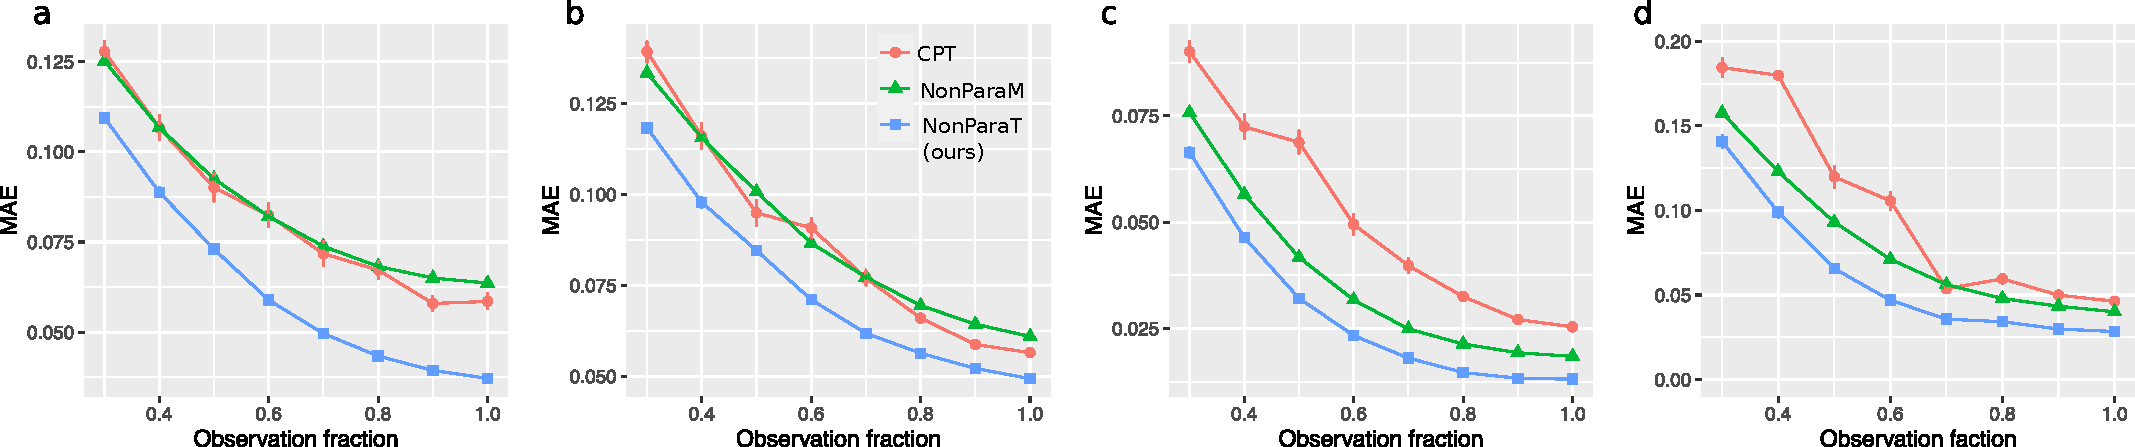
\includegraphics[width =\textwidth]{fig5-8v2.pdf}
    \end{center}
    \begin{itemize}
        \item Estimation error versus the observation fraction.
        \item Our method (NonparaT) achives the best performance.
    \end{itemize}
\end{frame}

\begin{frame}{Data application}
    \begin{center}
    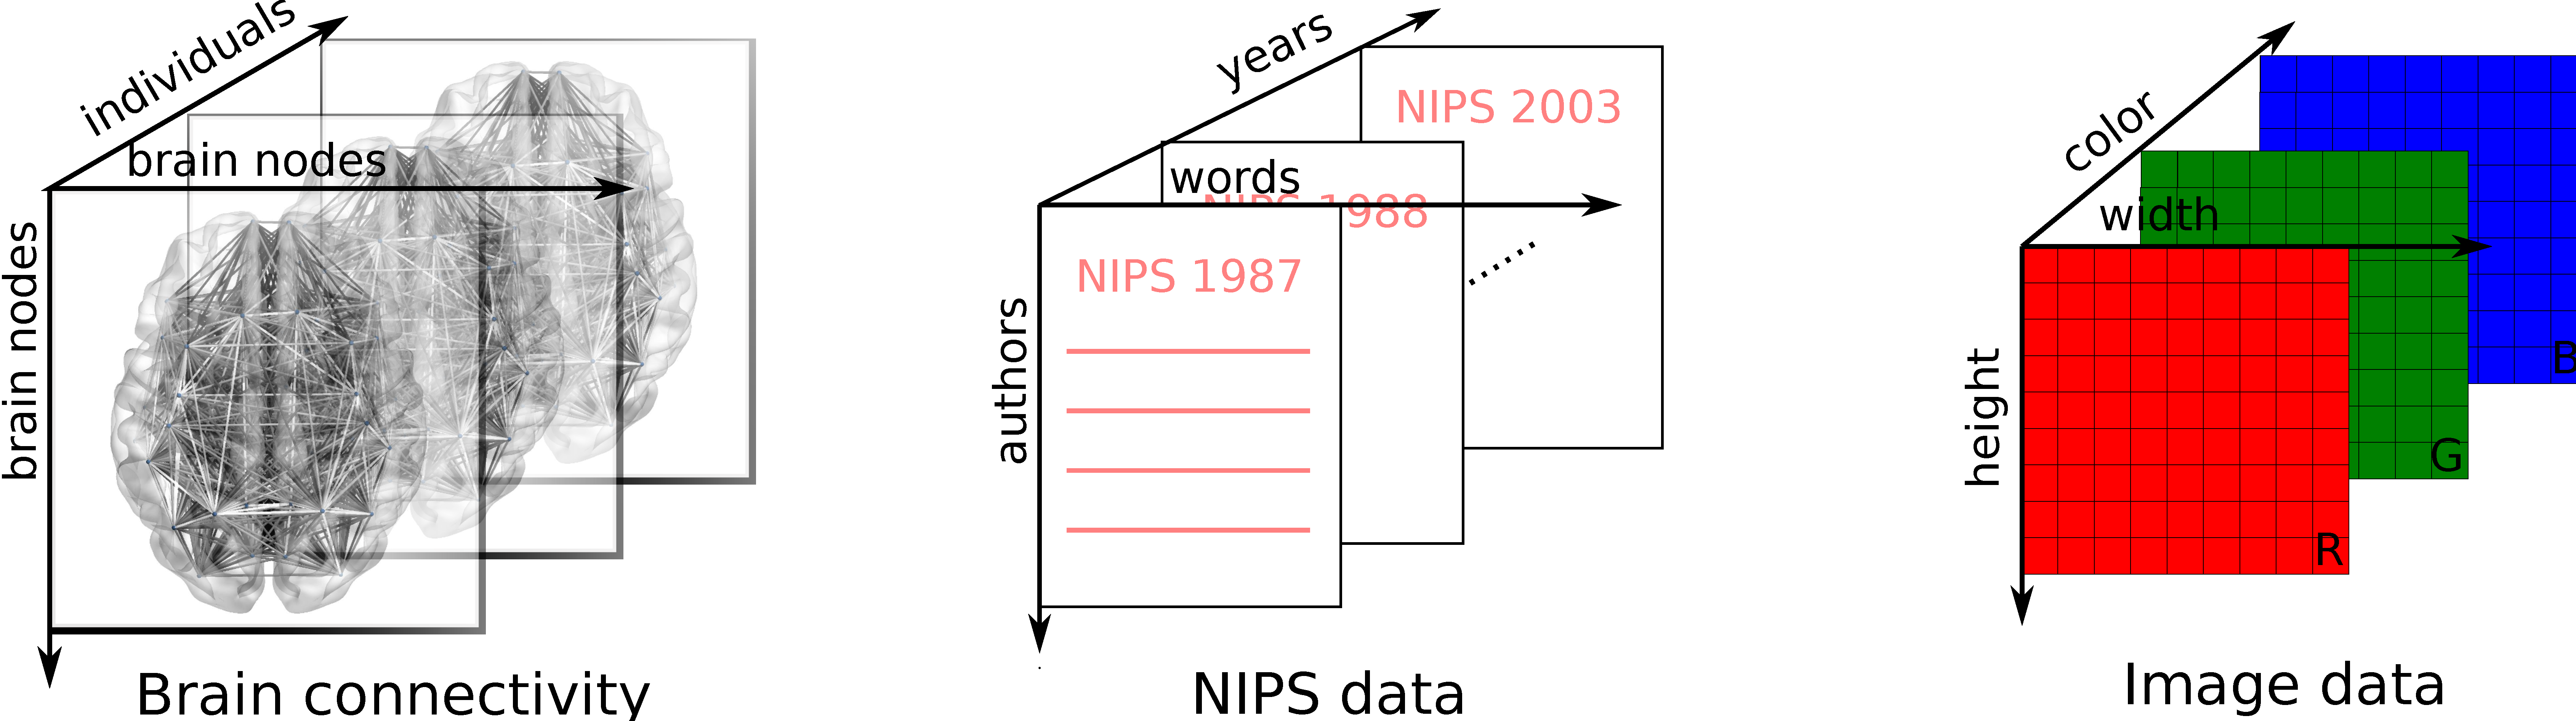
\includegraphics[width =\textwidth]{ndataset.pdf}
    \end{center}
\end{frame}

\begin{frame}{Data application: Brain connectivity}
\begin{columns}
\begin{column}{0.21\textwidth}
   \begin{center}
     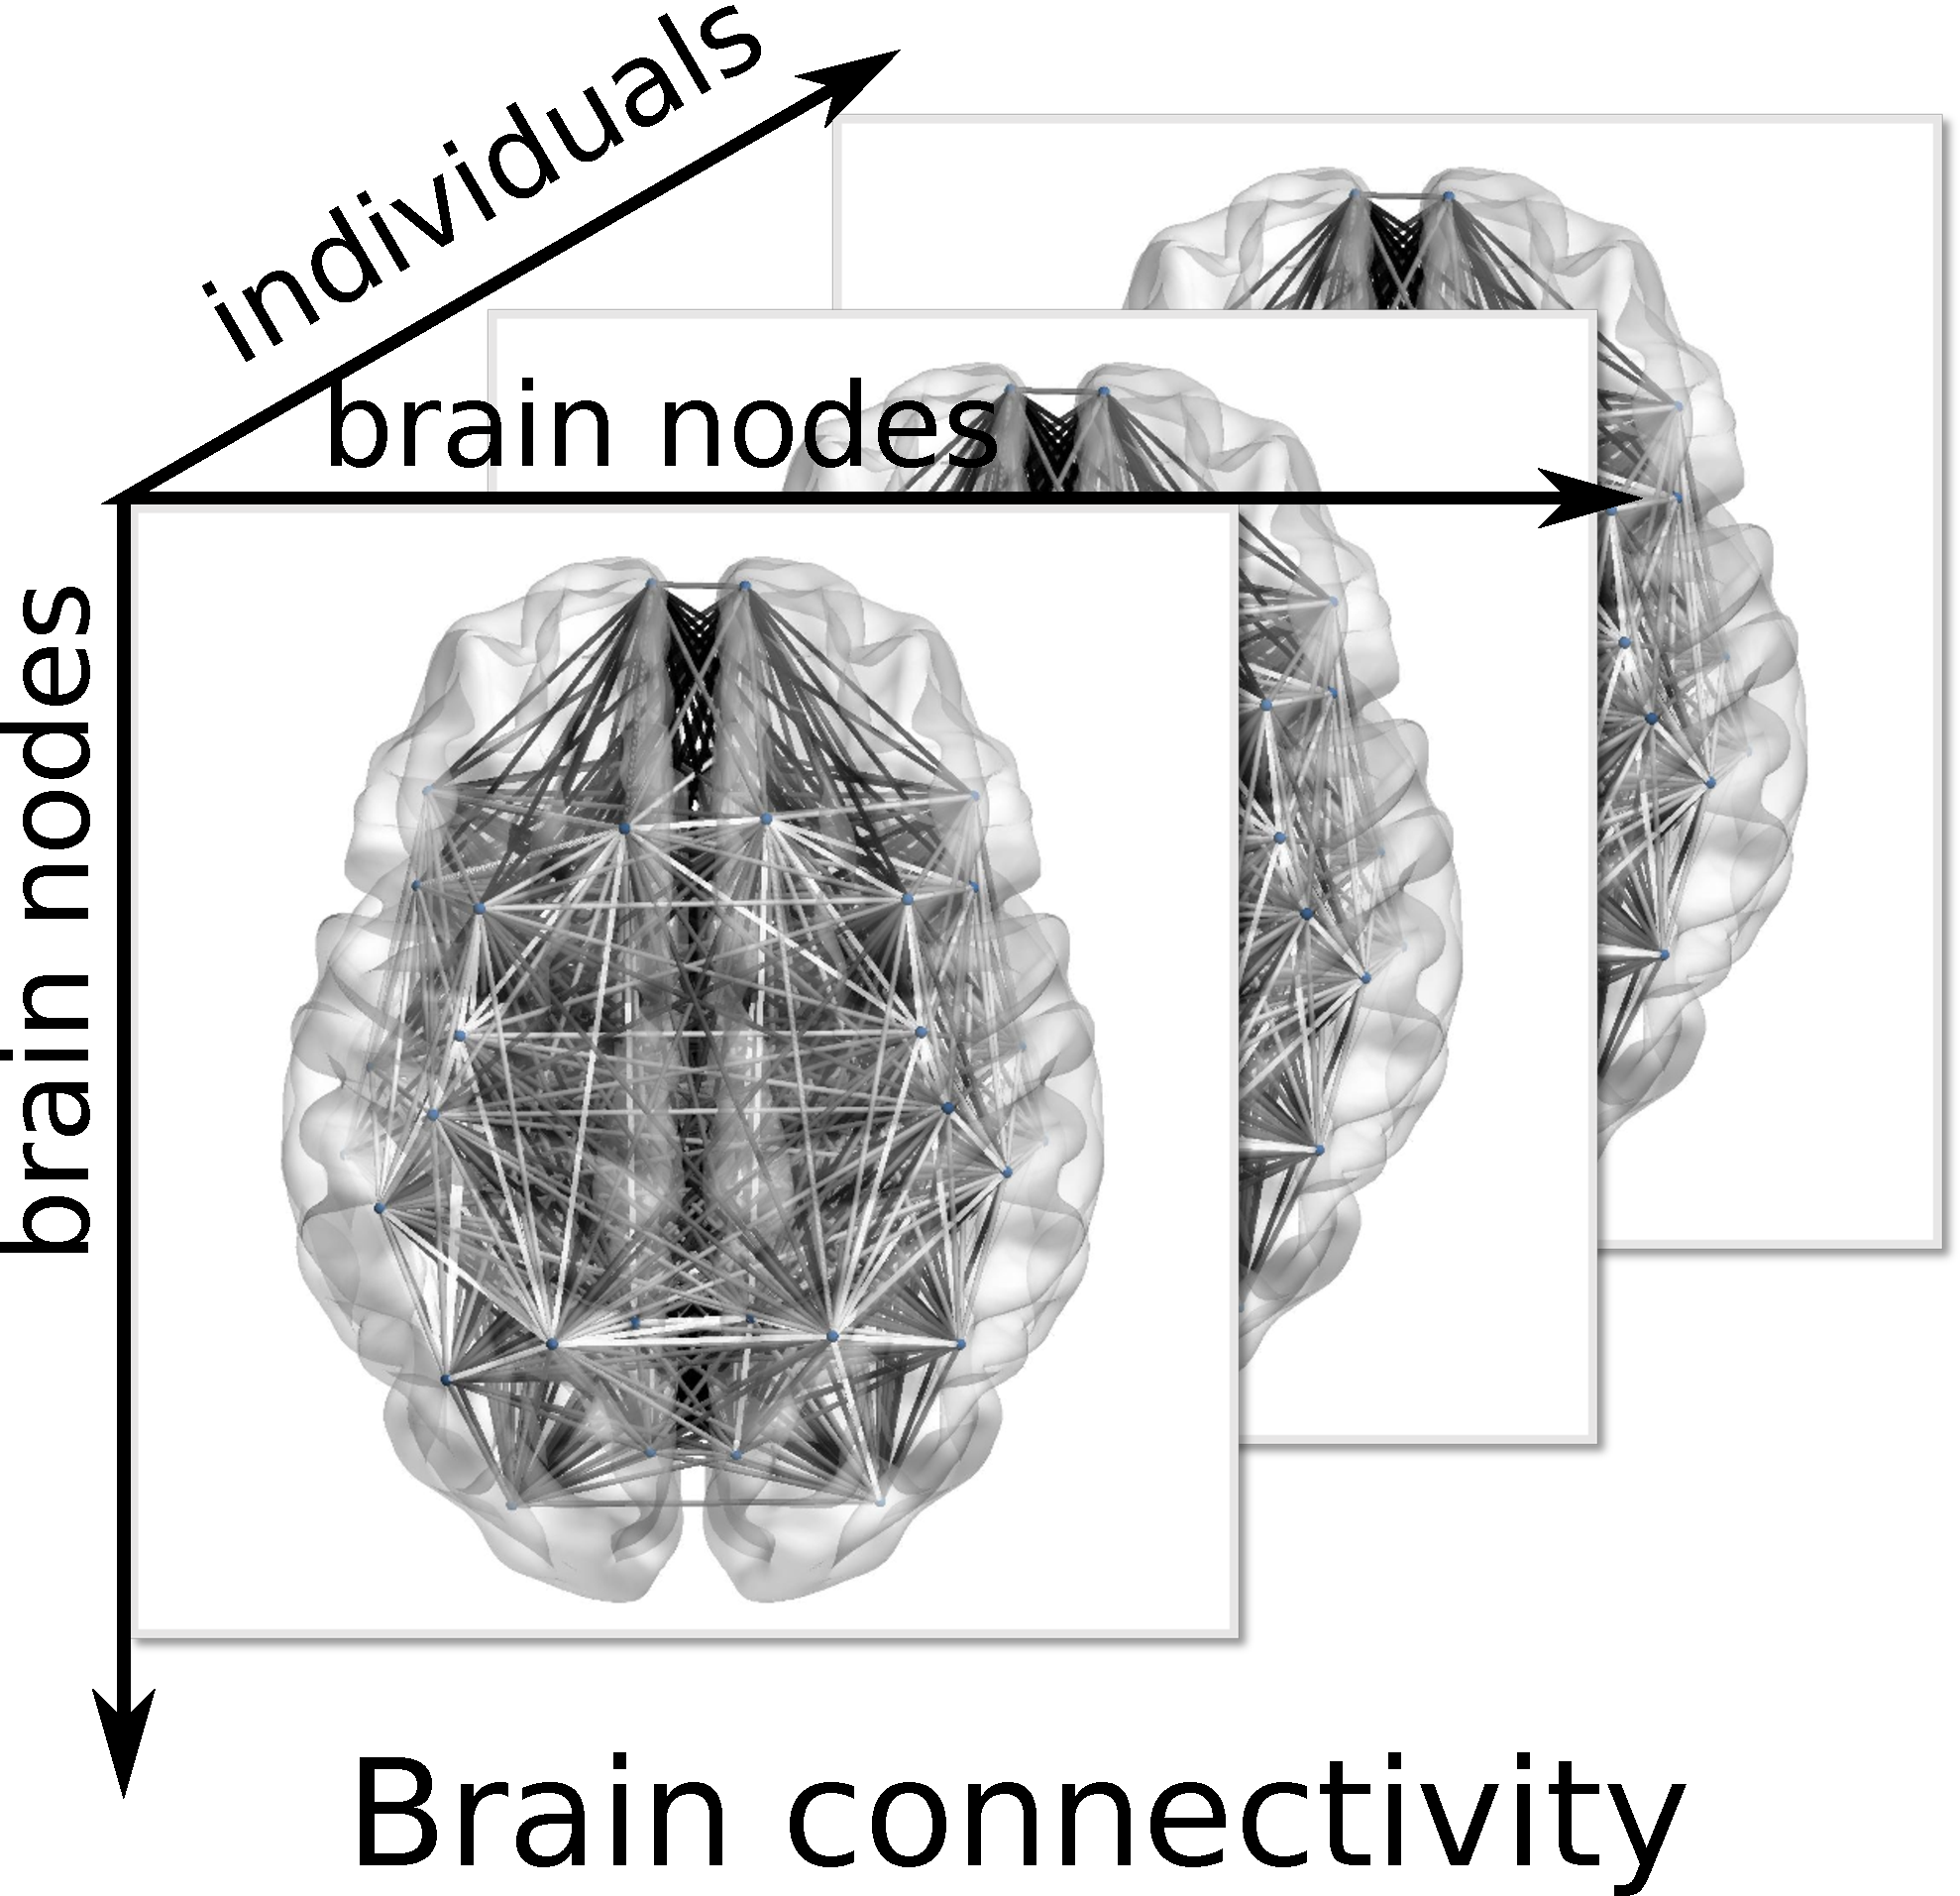
\includegraphics[width=\textwidth]{braindata.pdf}
     \end{center}
\end{column}
\begin{column}{0.7\textwidth} 
\begin{itemize}
    \item The MRN-114 human brain connectivity data consists of 68 brain regions for 114 individuals along with their IQ scores~\citep{wang2017bayesian}.
    \item  $\tY\in\{0,1\}^{68\times68\times114}.$
\end{itemize}
\end{column}
\end{columns}
\onslide<2->{
\begin{columns}
\begin{column}{0.6\textwidth}
 \begin{itemize}
     \item We examine the estimated signal tensor $\hat\Theta.$
     \item Top 10 brain edges based on regression analysis show inter-hemisphere connections.
 \end{itemize}
\end{column}
\begin{column}{0.4\textwidth} 
   \begin{center}
     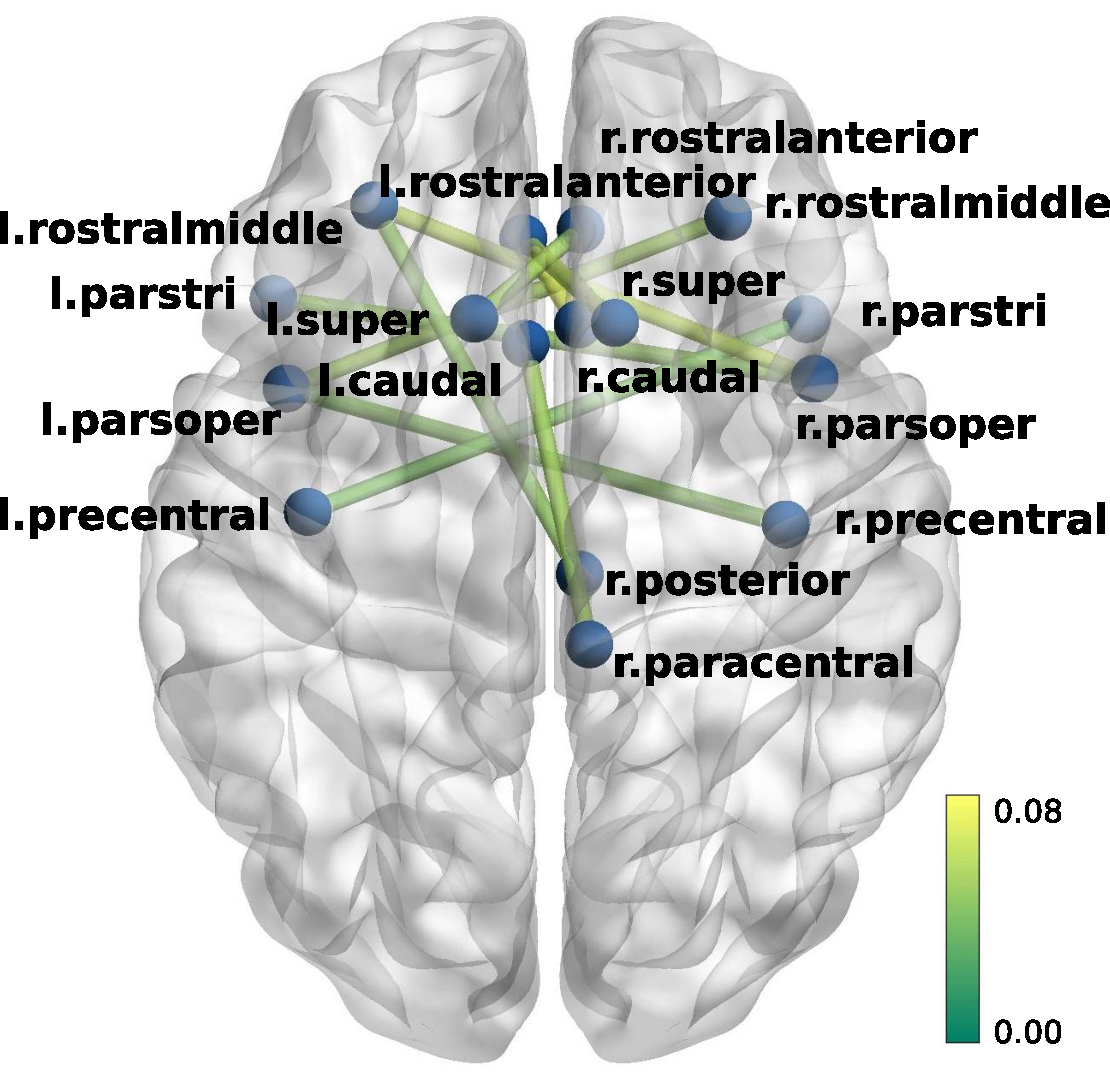
\includegraphics[width=\textwidth]{brainIQ.pdf}
     \end{center}
\end{column}
\end{columns}
}
\end{frame}



\begin{frame}{Data application: NIPS}
    \begin{columns}
\begin{column}{0.21\textwidth}
   \begin{center}
     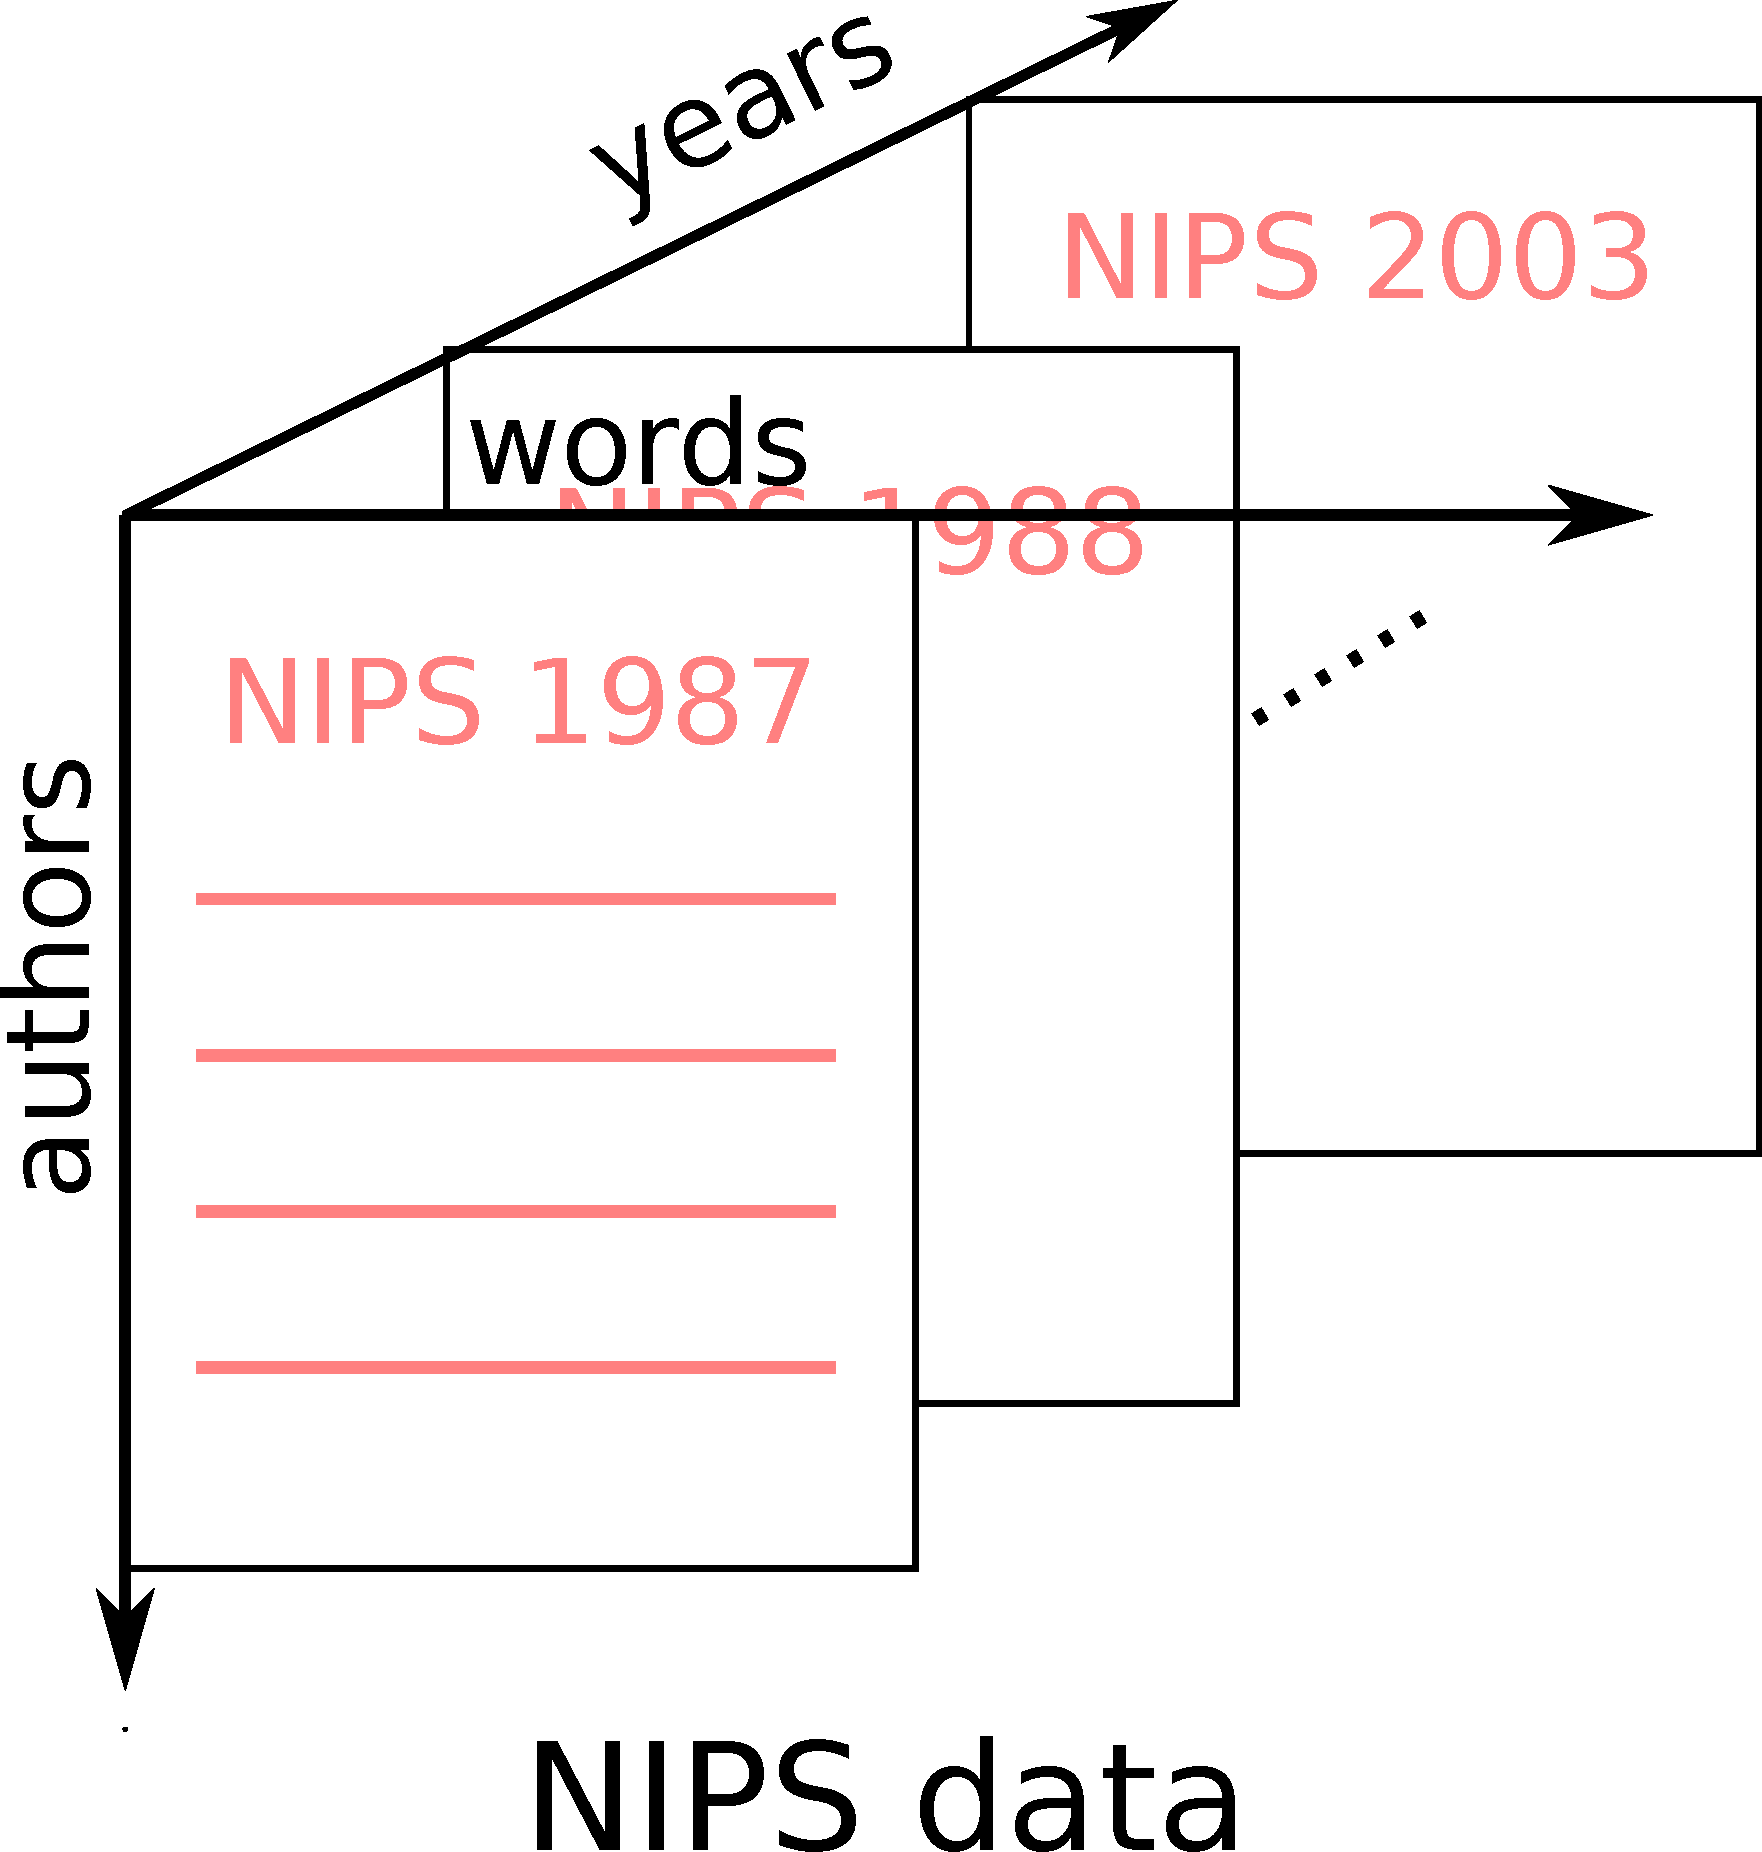
\includegraphics[width=\textwidth]{nipsdata.pdf}
     \end{center}
\end{column}
\begin{column}{0.7\textwidth} 
\begin{itemize}
    \item The NIPS dataset consists of word occurrence counts in papers published from 1987 to 2003~\citep{globerson2007euclidean}.
    \item Log transformation yields the dataset $\tY\in\mathbb{R}^{100\times200\times17}.$ 
\end{itemize}
\end{column}
\end{columns}

\onslide<2->{
\begin{columns}
\begin{column}{0.6\textwidth}
 \begin{itemize}
     \item We examine the estimated signal tensor $\hat\Theta.$
     \item Most frequent words is consistent with the active topics
     \item There are strong heterogeneity among word occurrences across authors and years.
 \end{itemize}
\end{column}
\begin{column}{0.4\textwidth} 
   \begin{center}
     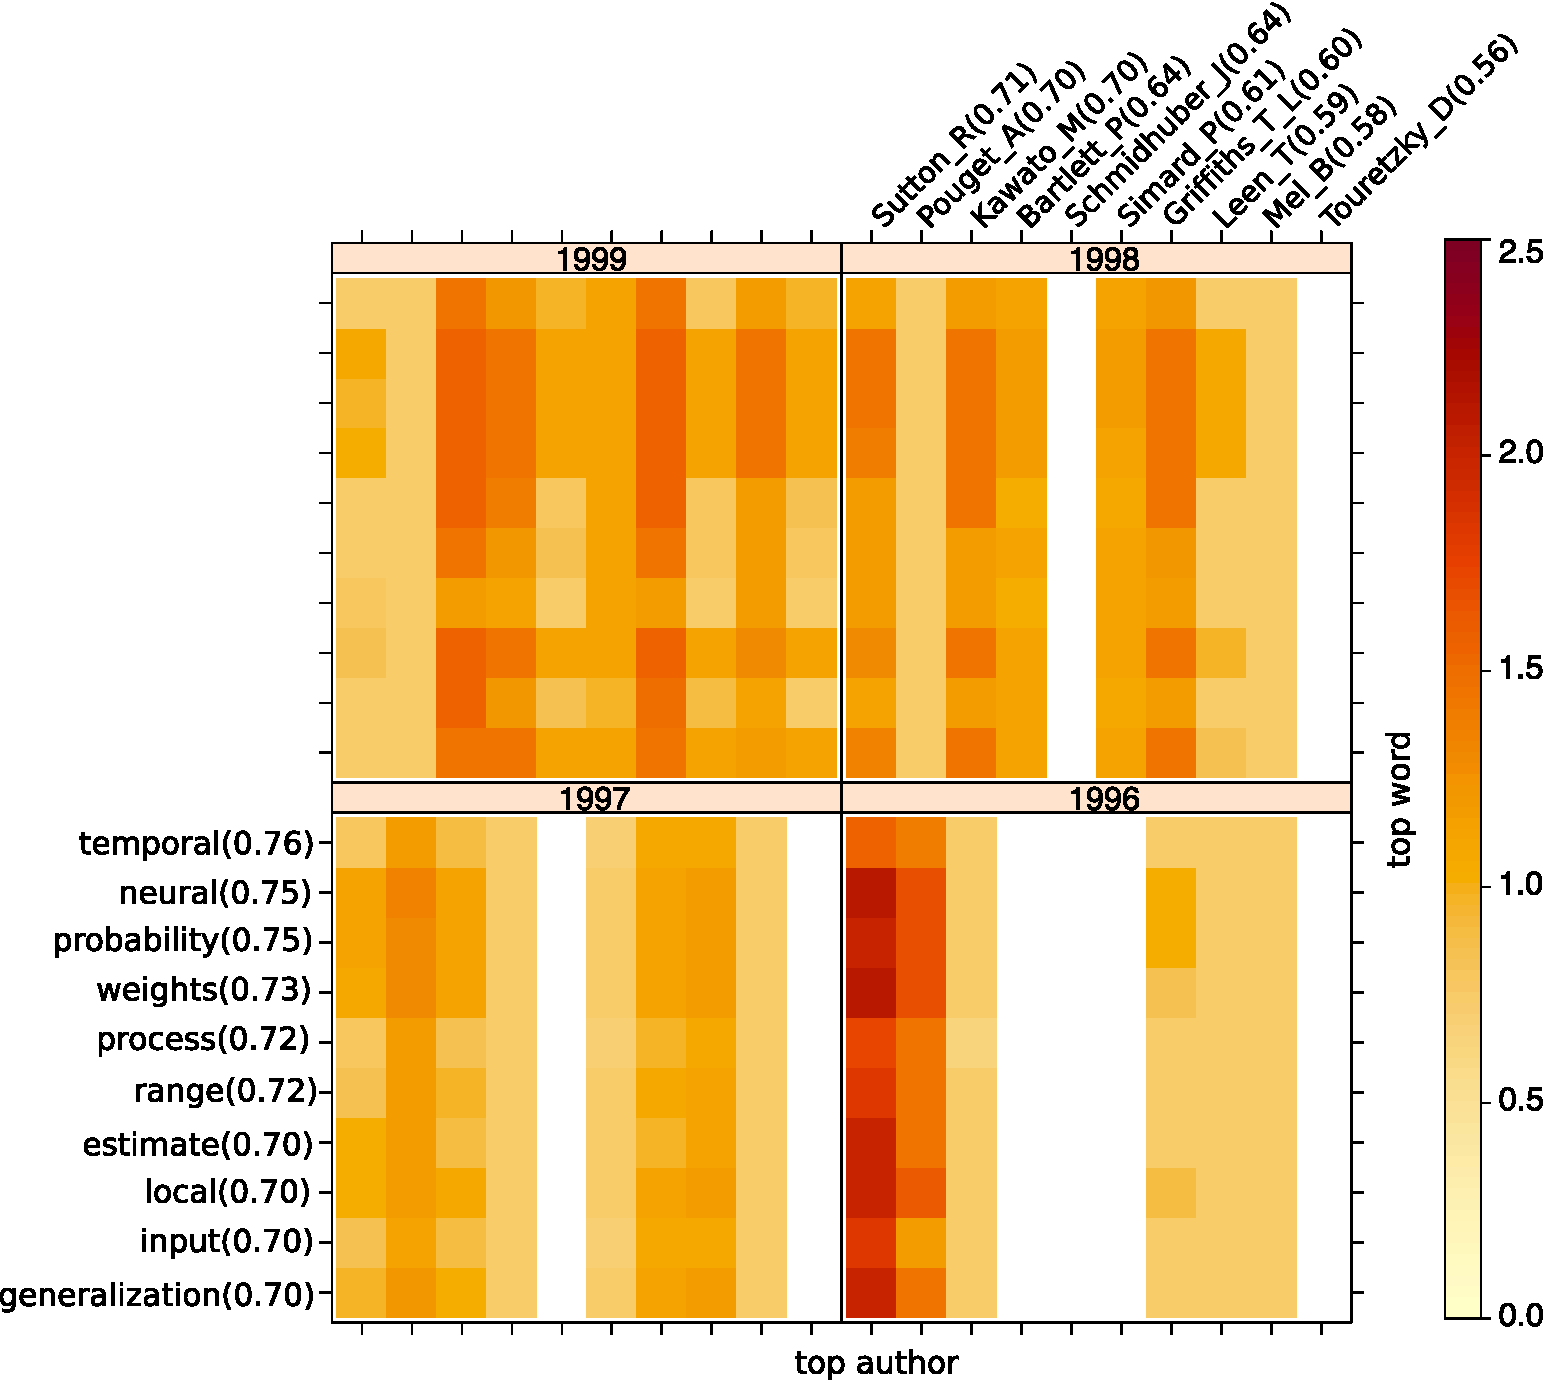
\includegraphics[width=\textwidth]{signal.pdf}
     \end{center}
\end{column}
\end{columns}
}
\end{frame}

\begin{frame}{Data application: Brain connectivity + NIPS}
      \begin{center}
     \begin{table}
    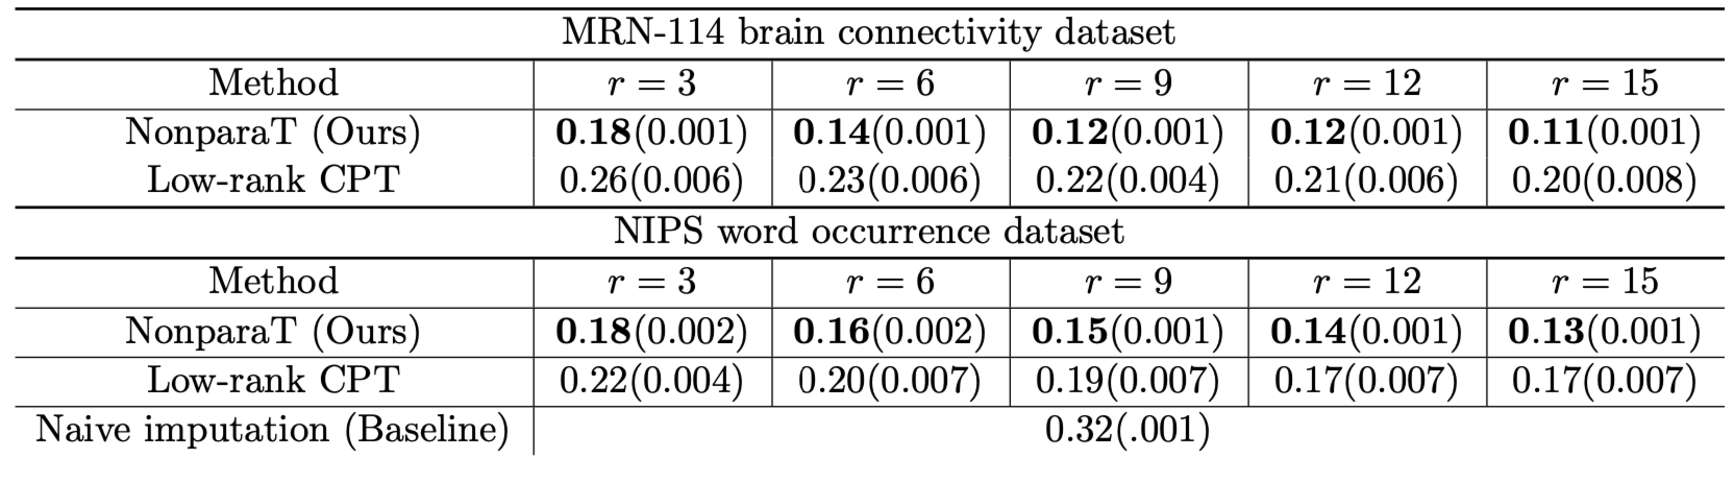
\includegraphics[width =\textwidth]{cvtable.pdf}
    \caption{MAE comparison in the brain data and NIPS data on cross-validation (5 repetitions 5 folds).  Standard errors are reported in parenthesis.}
    \end{table}
    \end{center}
\end{frame}

\begin{frame}{Data application: Image}
 \begin{columns}
\begin{column}{0.20\textwidth}
   \begin{center}
     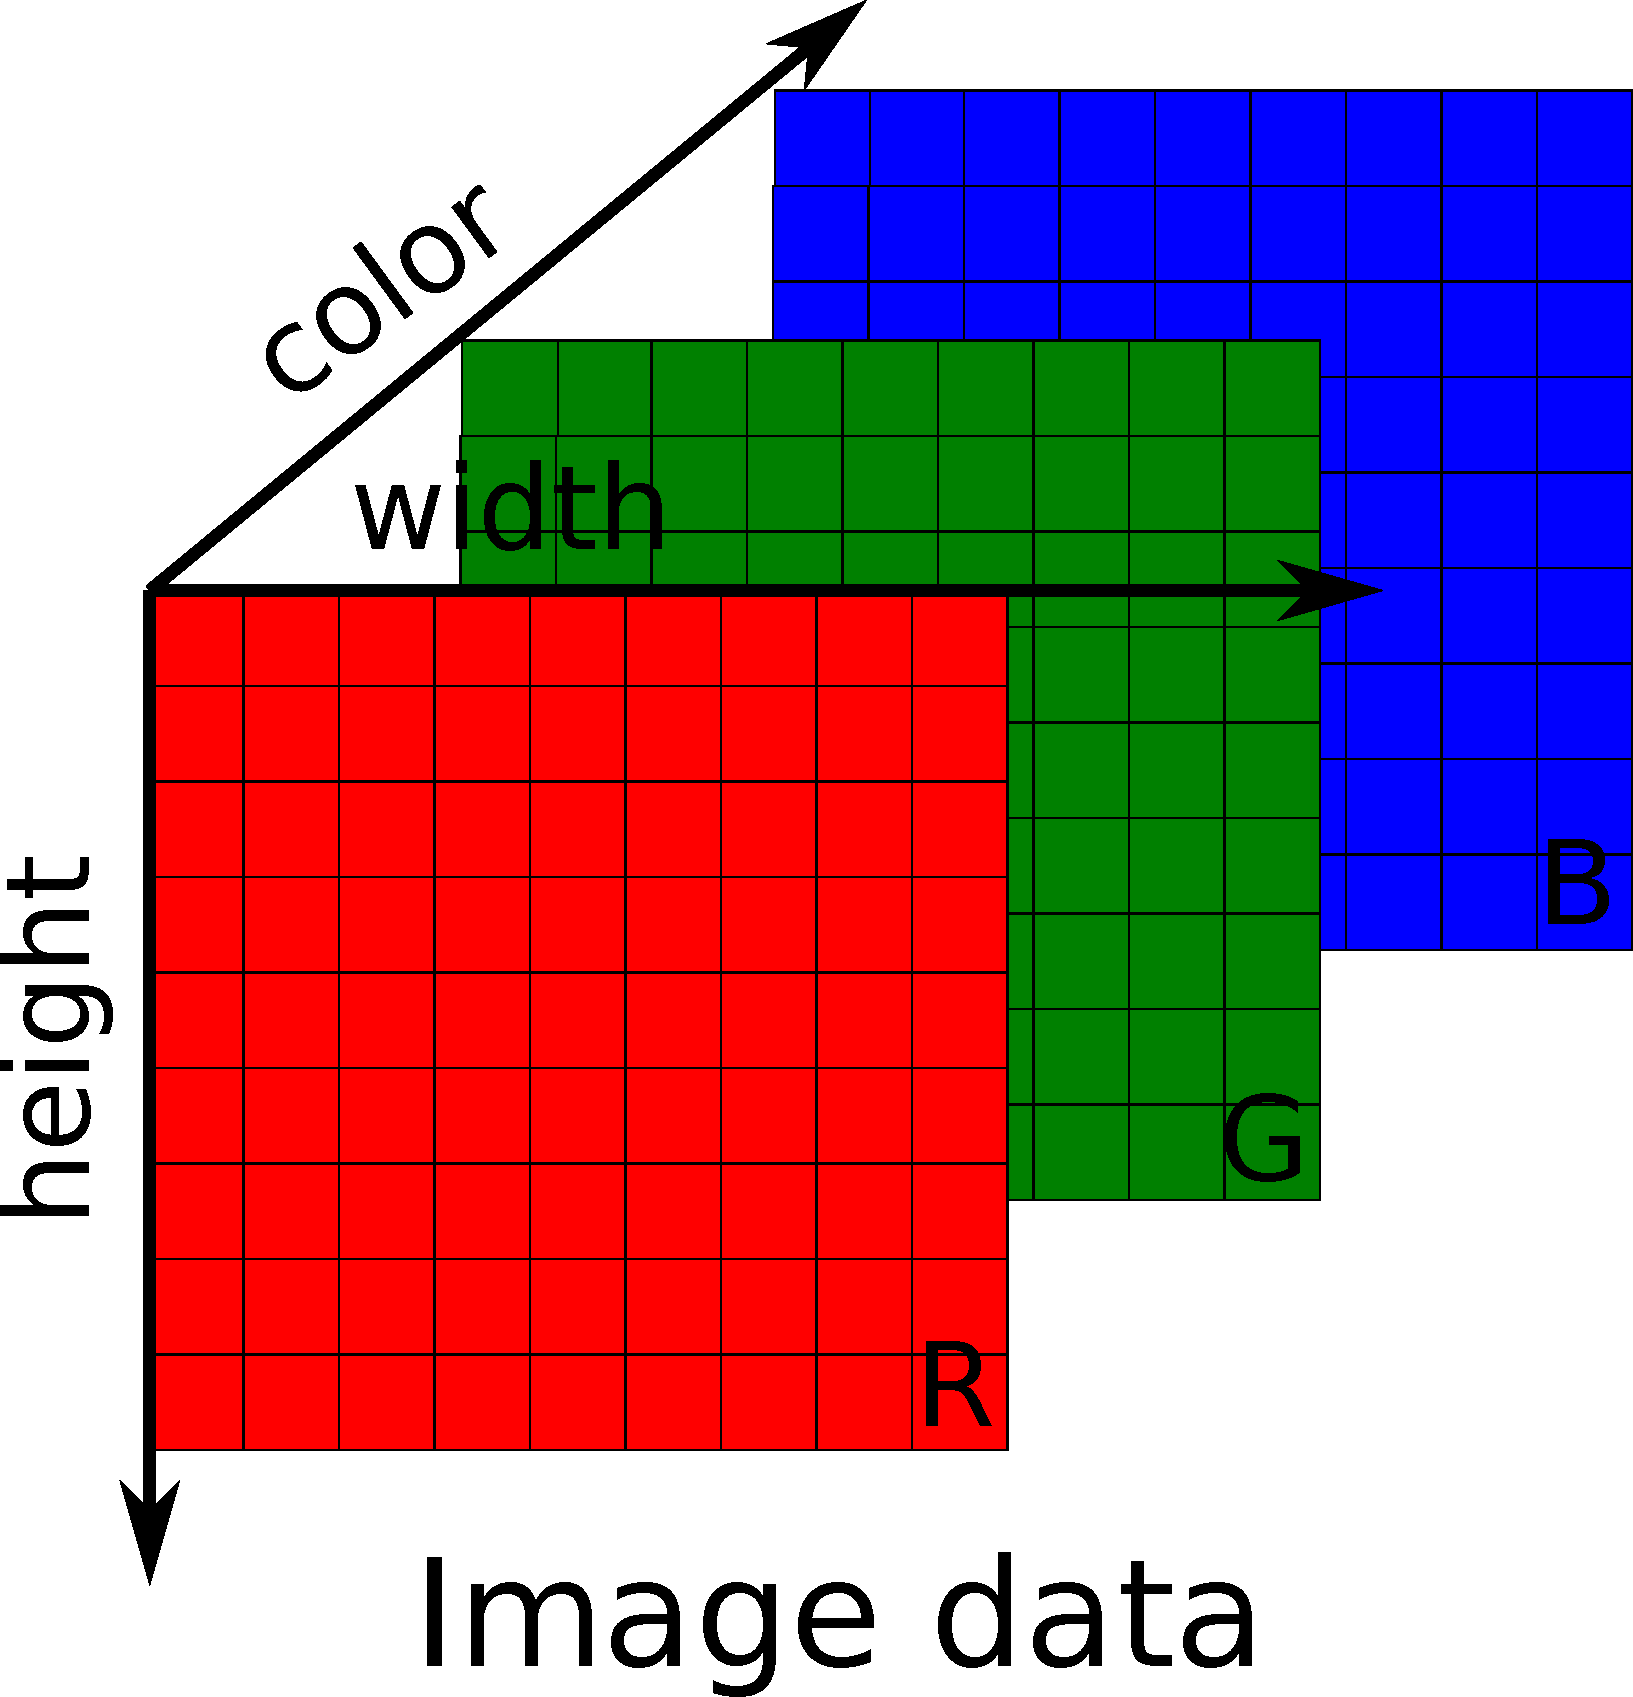
\includegraphics[width=\textwidth]{imgdata.pdf}
     \end{center}
\end{column}
\begin{column}{0.7\textwidth} 
\begin{itemize}
    \item The original data is from licensed google image file.
    \item  $\tY\in[0,1]^{217\times217\times3}.$ 
    \item We sample 50\% entries in the original image tensor and check completion performance.
\end{itemize}
\end{column}
\end{columns}
\onslide<2->{

      \begin{center}
    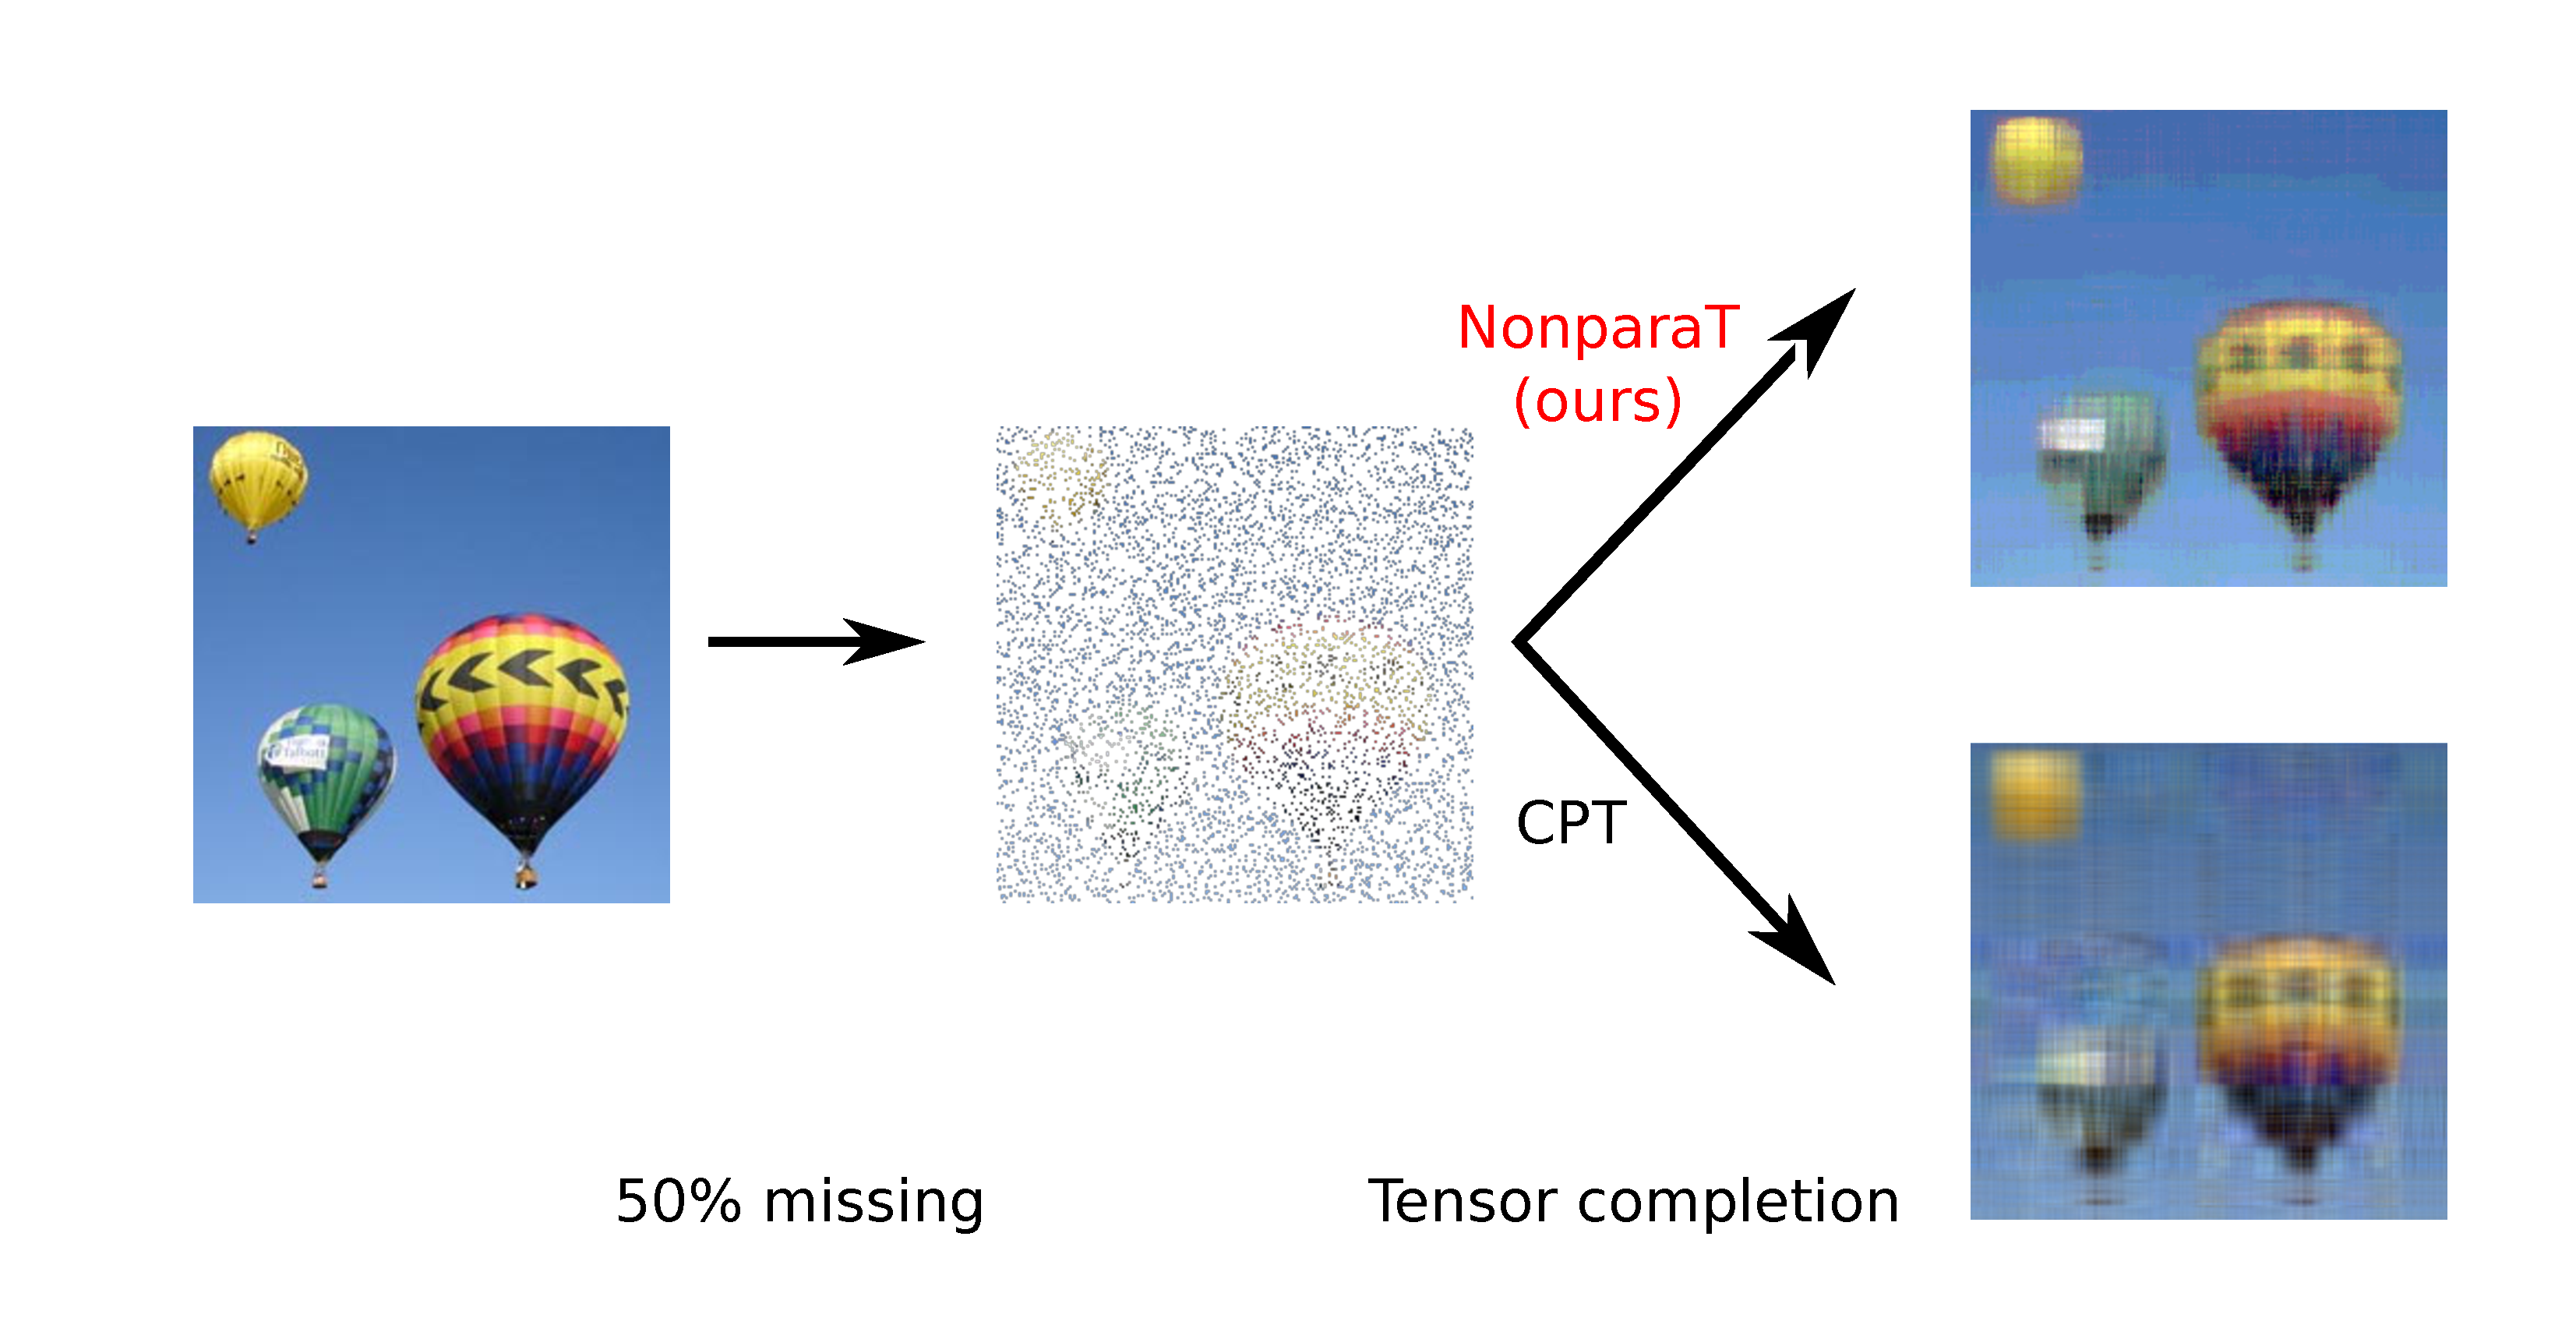
\includegraphics[width =\textwidth]{imageresult.pdf}
    \end{center}
    }
\end{frame}

\begin{frame}{Summary}
\begin{itemize}
    \item We have developed a completion method that can address {\color{red} both low- and high-ranknesss}  based on {\color{red}sign series representation}.
    \item {\color{red}Estimation error rates }and {\color{red}sample complexities} are established.
    \item Our approach has good interpretation and prediction performance in both simulations and data applications.
    \onslide<2->{
    \item Thank you!}
\end{itemize}
    
\end{frame}



\appendix
\begin{frame}{Appendix}
    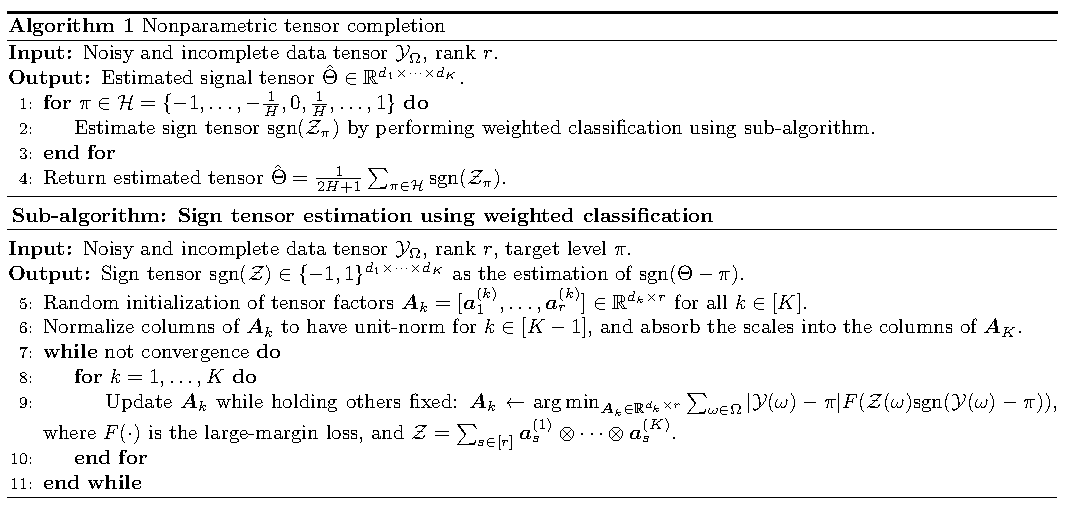
\includegraphics[width = \textwidth]{algorithm.pdf}
\end{frame}

\begin{frame}[allowframebreaks]
        \frametitle{References}
\bibliographystyle{apalike} 
\bibliography{tensor_wang}
\end{frame}



\end{document}
